% LuaLaTeX でコンパイルする: latexmk -lualatex KankyoJissu2026.tex
\documentclass{ltjsarticle}
\usepackage{graphicx}
\graphicspath{{figures/}}
\usepackage{amsmath}
\usepackage{ascmac}
\usepackage{bm}
\usepackage{comment}
\usepackage{setspace}
\usepackage{booktabs}
\usepackage{url}

\begin{document}

\title{環境化学実習（大気コース)\\ 2026年版}

\author{文責: 茂木}

\maketitle
本コースでは、{\bf 湿潤空気の熱力学}と{\bf 分子・熱の拡散移動現象}の理論を学び、それを応用して『水蒸気量』と『エアロゾル数濃度』の自動測定装置を製作する。実験では、物理量センサーとコンピュータのインターフェースとなる{\bf アナログ電子回路}を製作して動作検証をする。データ解析では、装置のなかで起こっている物理現象をシミュレーションする{\bf 順問題モデル}を使って、装置の信号から知りたい物理量を推定するための{\bf 逆問題モデル}を導出する。自作装置による連続観測を１週間程度実施し、観測信号から導出される水蒸気量やエアロゾル数濃度を、市販の測定器による観測値と比較して検証する。データ解析ではプログラミング言語Pythonを用いる\footnote{Python開発環境パッケージ（MiniforgeまたはAnaconda）を自分のノートPCにインストールしておいてください。}。2026年版では、計測制御のソフトウェアをPythonで作り直し、エアロゾル粒子の活性化の微物理（\ref{sec:activation}節）と、シミュレーションベース推論による推定法（\ref{sec:sbi}節）の説明を加えた。観測装置開発の全ての工程（理論・試作・データ解析）を俯瞰しておくことは、既存装置の仕組みを理解したり、新規の開発を試みる際の助けになると思われる。

\tableofcontents


\section{湿潤空気の熱力学}
熱力学は、多数の原子・分子から構成される系の性質や挙動が、温度・圧力・密度・組成という少数の巨視的パラメータ（熱力学変数）のみで記述できるという経験事実に基づいている。系の内部が空間的に一様であるならば、その系の温度・圧力・密度・組成といった熱力学変数が定義でき、熱力学理論を適用可能である。例えば、実大気中で気温・気圧・組成が一様な空気塊については、それを一つの系とみなした熱力学理論を適用してよい。湿潤空気の熱力学では、水蒸気の相転移に伴う潜熱の放出や吸収の影響も考慮される。上昇する湿潤空気塊の温度が低下し雲粒が発生・成長する現象は、湿潤空気塊を孤立系とみなした巨視的な熱力学と、雲粒周辺における微視的な分子・熱の拡散法則により記述できる。本演習では、大気中でエアロゾルから雲粒が発生し成長する現象をフラスコ内で模擬し、その現象を利用して水蒸気とエアロゾルの測定することを試みる。

まず、水蒸気を含んだ空気（湿潤空気）の熱力学に用いる変数の定義を説明する。

\subsection{湿潤空気の状態の記述法}
空気は、地球大気中の温度と圧力の条件下でほぼ理想気体であり、熱力学変数である圧力$p\,[\rm{Pa}]$、体積$V\,[\rm{m^{3}}]$、温度$T\,[\rm{K}]$の間に以下の理想気体の状態方程式が成り立つ。

\begin{equation}\label{eq:1}
 pV=nR^{*}T 
\end{equation}
ここで$n\,[\rm{mol}]$は気体分子のモル数、$R^{*}\,[\rm{J\,K^{-1}\,mol^{-1}}]$は一般気体定数である。複数の分子種からなる理想気体では、各分子種の分圧はモル分率に比例するので、空気塊を構成する各分子種 $(i = 1,2,\dots, k)$について、状態方程式
\begin{equation}\label{eq:2}
 p_{i}V=n_{i}R^{*}T 
\end{equation}
が成立する。 \eqref{eq:1}と\eqref{eq:2} は互いに分圧とモル数の加法性
\begin{equation}\label{eq:3}
 p=\sum_{i=1}^{k}p_{i}\,, \ \ n=\sum_{i=1}^{k}n_{i},
\end{equation}
で結ばれている。大きさが決まっていない大気中の空気塊を、系の大きさに比例するモル数や体積など変数（示量性変数）を使って記述するのは不便である。そのため、状態方程式\eqref{eq:2}において、示量性変数のモル数$n$と体積$V$の代わりに、示強性変数である質量密度$\rho\,[\rm{kg\,m^{-3}}]$を用いるようにしたい.。

まず、各分子種$i$についての状態方程式を導出しておく。分子数$n_{i}\,[\rm{mol}]$の質量を$m_{i}\,[\rm{kg}]$とし、分子種$i$についての気体定数$R_{i}\,[\rm{J\,K^{-1}\,kg^{-1}}]$を、$R^{*}$を分子量$M_{i}$で割った量として定義する.。
\begin{equation}\label{eq:4}
 R_{i}=\frac{n_{i}R^{*}}{m_{i}}=\frac{R^{*}}{M_{i}},
\end{equation}
分子種$i$の質量密度$\rho_{i}\,\rm{[kg\,m^{-3}]}$は、定義より
\begin{equation}\label{eq:5}
 \rho_{i}=\frac{m_{i}}{V}
\end{equation}
である。式\eqref{eq:4}、\eqref{eq:5}を式\eqref{eq:2}に代入すると、分子種$i$の状態方程式は
\begin{equation}\label{eq:6}
 p_{i}=\rho_{i}R_{i}T 
\end{equation}
と書ける。次に、混合理想気体の状態方程式を導出する。まず、分子種$i\,(i = 1,2,\dots, k)$のモル分率$f_{i}$
\begin{equation}\label{eq:7}
 f_{i}=\frac{n_{i}}{\sum_{i=1}^{k}n_{i}} 
\end{equation}
によって平均分子量$\overline{M}$を表すと、
\begin{equation}\label{eq:8}
 \overline{M}=\frac{\sum_{i=1}^{k}m_{i}}{\sum_{i=1}^{k}n_{i}}=\frac{\sum_{i=1}^{k}n_{i}M_{i}}{\sum_{i=1}^{k}n_{i}}=\sum_{i=1}^{k}f_{i}M_{i}
\end{equation}
となる。一方で、各分子種$i$の状態方程式\eqref{eq:2}を$k$個の分子種について足し合わせると、
\begin{equation}\label{eq:9}
 pV=\sum_{i=1}^{k}m_{i}\overline{R}T 
\end{equation}
とかける。ここで$\overline{R}\,[\rm{J\,K^{-1}\,kg^{-1}}]$は以下のように定義される混合気体の気体定数である。
\begin{equation}\label{eq:10}
 \overline{R}=\frac{\sum_{i=1}^{k}n_{i}R^{*}}{\sum_{i=1}^{k}m_{i}}=\frac{R^{*}}{\overline{M}}
\end{equation}
ここで式\eqref{eq:10}の最後の変形では式\eqref{eq:8}を用いた。式\eqref{eq:9}の両辺を体積$V$で割ると、混合気体の状態方程式
\begin{equation}\label{eq:11}
 p=\rho\overline{R}T 
\end{equation}
を得る。ここで式\eqref{eq:11}において密度$\rho$は
\begin{equation}\label{eq:12}
 \rho=\frac{1}{V}\sum_{i=1}^{k}m_{i} 
\end{equation}
として定義した。

地球大気の主要成分のなかで、例外的に水蒸気はモル分率が時空間的に著しく変動する（変動範囲は0～5\%程度）。そのため気象学では、空気を乾燥空気と水蒸気の２つの分子種のから成る混合気体として扱うことが多い。乾燥空気は安定な主要成分である$\rm{N_{2}}\,(78.08\%),\ \rm{O_{2}}\,(20.95\%),\ \rm{Ar}\,(0.93\%),\ \rm{CO_{2}}\,(\sim0.04\%)$の4分子種の混合気体として定義される。( )内の数字は乾燥空気中の各分子種のモル分率である。乾燥空気の分圧、密度、気体定数をそれぞれ記号$p_{d},\ \rho_{d},\ R_{d}$で表し、水蒸気の分圧、密度、気体定数はそれぞれ$e,\ \rho_{v},\ R_{v}$で表せば、各成分の状態方程式は
\begin{equation}\label{eq:13}
 p_{d}=\rho_{d}R_{d}T,
\end{equation}
\begin{equation}\label{eq:14}
 e=\rho_{v}R_{v}T,
\end{equation}
と書ける。ここで、湿潤空気の気圧$p$は
\begin{equation}\label{eq:15}
 p=p_{d}+e,
\end{equation}
である。水蒸気混合比$q_{v}\,[-]$は、同じ空気塊内の水蒸気と乾燥空気の質量比として定義される。([-]は単位が無次元であることを示す) すなわち
\begin{equation}\label{eq:16}
 q_{v}=\frac{\rho_{v}}{\rho_{d}},
\end{equation}
である。密度の代わりに圧力で$q_{v}$を表すと
\begin{equation}\label{eq:17}
 q_{v}=\epsilon\frac{e}{p_{d}}=\epsilon\frac{e}{p-e}\approx\epsilon\frac{e}{p},
\end{equation}
ただし$\epsilon\,[-]$は水と乾燥空気の分子量の比であり、
\begin{equation}\label{eq:18}
 \epsilon=\frac{M_{v}}{M_{d}},
\end{equation}
で定義される定数$(= 0.622)$である。乾燥空気分圧$p_{d}$と全圧$p$の差は大きくても$2 \sim 3\%$であるため、本演習では特に断らない限り、式\eqref{eq:17}最右辺の近似を認めることにする。
\\
\begin{itembox}[l]{\bf{例題1.}}
水蒸気の気体定数$R_{v}$を$[\rm{J\,K^{-1}\,kg^{-1}}]$の単位で求めよ。水の平均分子量は$M_{v}=18.02[\rm{g\,mol^{-1}}]$である。
答：$R_{v}=461.4[\rm{J\,K^{-1}\,kg^{-1}}]$
\end{itembox}
\\
\begin{itembox}[l]{\bf{例題2.}}
乾燥空気の平均分子量$M_{d}\,\rm{[g\,mol^{-1}]}$と気体定数$R_{d}\,\rm{[J\,K^{-1}\,kg^{-1}]}$を4つの主成分$\rm{N_{2}\,(28.013)}$, $\rm{O_{2}\,(31.999)}$, $\rm{Ar \,(39.948)}$, $\rm{CO_{2}\,(44.010)}$を考慮して求めよ。 各々の分子種の平均分子量$\rm{[g\,mol^{-1}]}$は( )内に示した。
答：$M_{d}=28.97[\rm{g\,mol^{-1}}]$, $R_{d}=287.0[\rm{J\,K^{-1}\,kg^{-1}}]$
\end{itembox}
\\
\\

ここで、水蒸気量の４通りの表現法である水蒸気圧$e$、水蒸気混合比$q_{v}$、露点温度$T_{d}$、飽和比$S$それぞれの定義と相互関係を示しておく。このために、後に1.3節で詳しく説明する平衡水蒸気圧$e_{s}(T)$を用いる\footnote{表記$e_{s}(T)$は、平衡水蒸気圧$e_{s}$が温度$T$の関数であることを意味する。}。水蒸気圧$e$が与えられたとき、露点温度$T_{d}$は、温度$T$についての方程式
\begin{equation}\label{eq:19}
 e_{s}(T)=e
\end{equation}
の解として求められる。水蒸気圧$e$を水蒸気混合比$q_{v}$と気圧$p$で表すと、式\eqref{eq:19}は
\begin{equation}\label{eq:20}
 e_{s}(T_{d})=\frac{q_{v}}{\epsilon}p
\end{equation}
となる。式\eqref{eq:20}から、露点温度$T_{d}$は水蒸気混合比$q_{v}$と気圧$p$に依存することがわかる。一方、飽和比$S$は、
\begin{equation}\label{eq:21}
 S=\frac{e}{e_{s}(T)}
\end{equation}
として定義される。飽和比を百分率で表したものは相対湿度とも呼ばれる。４種類の水蒸気量の表現法（水蒸気圧$e$、水蒸気混合比$q_{v}$、露点温度$T_{d}$、飽和比$S$）のうち、空気塊の運動に伴い容易に変化しうる温度や気圧に依存しないのは水蒸気混合比だけである。そのため、本演習では水蒸気量の観測データを水蒸気混合比$q_{v}$として表すことにする。

以上で湿潤空気の記述に必要な変数は全て定義した。次に熱力学理論の説明に入る。

\subsection{熱力学第１法則}
系が外界から受け取る熱を$Q\,[\rm{J}]$、系の内部エネルギーを$U\,[\rm{J}]$、系が外界に対してする仕事を$W\,[\rm{J}]$とする。これらの量の時間変化には、エネルギーの保存則から
\begin{equation}\label{eq:22}
 \frac{dQ}{dt}=\frac{dU}{dt}+\frac{dW}{dt},
\end{equation}
の関係が成り立つ。ここで$Q$は分子論的に乱雑で秩序のない形式のエネルギーの移動量である。一方、$W$は分子論的に秩序のある形式のエネルギーの移動量であり,、抵抗力に抗って物を動かす力学的なエネルギーでも良いし電磁気的なエネルギーでもよい\footnote{分子論的に秩序のないエネルギー移動である熱$Q$と分子論的に秩序のあるエネルギ−移動である仕事$W$の間の変換には熱力学第２法則による強い制約があるため、これら二つの形式のエネルギー移動量は常に分けて考える。}。$U$は系のエネルギー保持量を表している。$U$の中身が熱エネルギーなのか、または何らかの秩序ある形式のエネルギーなのかは任意である。式\eqref{eq:22}は熱力学第１法則と呼ばれ、どんな形式のエネルギーも総量は保存され、系と外界との間の移動量と系の保持量の収支は釣り合うことを意味している．

この1.2節の目的は、熱の移動量$Q$を、直接観測することが難しい$U$や$W$の関数としてではなく、観測可能な熱力学状態量である温度$T$、圧力$p$、単位質量当たりの体積$v$（密度$\rho$の逆数）の関数として表すことである\footnote{この表現から、応用で特に重要な「断熱変化」の式を得る。}。

ある物体に力$\bf{f}\,[\rm{N}]$を加えて$d{\bf x}/dt\,[\rm{m\,s^{-1}}]$の速度で動かす時、物体になされる仕事$W$の時間微分は、
\begin{equation}\label{eq:23}
 \frac{dW}{dt}={\bf f}\cdot \frac{d{\bf x}}{dt},
\end{equation}
と表される\footnote{ベクトル量はボールド体で表記する。}。ただし{\bf x}は物体の位置ベクトルである。

空気塊に熱力学第１法則を適用する準備をする。まず、膨張する空気塊が外界とやり取りする仕事$dW/dt$はどのように表されるだろうか？
空気塊の表面の面積要素$ds\,[\rm{m^{2}}]$を考え、単位面積当たりに作用する力を${\bf f}\,[\rm{N m^{-2}}]$、面積要素の位置ベクトルを${\bf l}\,[\rm{m}]$とすると、空気塊が外界に対してなす仕事は一般に
\begin{equation}\label{eq:24}
 \frac{dW}{dt}=\int{\bigg (}{\bf f}\cdot \frac{d{\bf l}}{dt}{\bigg )}\,ds,
\end{equation}
と表される。ここで積分は空気塊の表面全体にわたって行う。

ここでは、式\eqref{eq:24}で表される仕事の特別な場合として，膨張がゆっくりと起こる場合を考えよう．「ゆっくり」というのは，膨張の最中でも空気塊内の圧力の均一性が保たれるほどにゆっくりという意味である\footnote{この条件は膨張の速さ$| d{\bf l}/dt |$が音速（すなわち圧力波の伝搬速度）よりもずっと遅い場合にあてはまる．}．膨張がゆっくり起こるとき，その過程の各瞬間において，空気塊内部の圧力と密度はともに空間的に一様なので、状態方程式により温度も空間的に一様である。そのため、各瞬間に外界に微小な仕事$dW$をしたことによる影響は空気塊の全域に一様にかつ同時に起こる。このように、ゆっくりとした変化過程のことを{\bf 準静的過程}と呼ぶ\footnote{準静的過程の系の時間変化の記述には熱力学理論を使うことができる。一方、準静的でない系の時間変化の記述には熱力学理論はそのまま使えない。非平衡熱力学という進んだ理論体系が必要である。}。このとき、空気塊の表面の単位面積に作用する力${\bf f}$は, 方向は面積要素$ds$に垂直で大きさは外界の気圧$p$に等しくなる．面積要素$ds$に垂直な単位ベクトルを${\bf n}$とおけば、
\begin{equation}\label{eq:25}
 {\bf f}=p{\bf n},
\end{equation}
と表される。式\eqref{eq:24}に式\eqref{eq:25}を代入して、さらに体積の変化速度$dV/dt$の数学的定義を考慮すると
\begin{equation}\label{eq:26}
 \frac{dW}{dt}=p\frac{dV}{dt},
\end{equation}
となる。圧縮する場合は位置ベクトルの変化$d{\bf l}$の向きが面積要素$ds$に対して内側向きになるため$dV$の符号が負になる。

時刻$t_{0}$から$t_{1}$にかけて体積が$V_{0}$から$V_{1}$まで膨張したとき，系から外界に対して行う仕事量は，式\eqref{eq:26}の積分により
\begin{equation}\label{eq:27}
 W=\int_{t_{0}}^{t_{1}}{\bigg (}\frac{dW}{dt}{\bigg )}dt=\int_{t_{0}}^{t_{1}}p{\bigg (}\frac{dV}{dt}{\bigg )}dt=\int_{V_{0}}^{V_{1}}p\,dV,
\end{equation}
と書ける。式\eqref{eq:26}を式\eqref{eq:22}に用いると,、空気塊についての熱力学第１法則は
\begin{equation}\label{eq:28}
 \frac{dQ}{dt}=\frac{dU}{dt}+p\frac{dV}{dt},
\end{equation}
と書ける。これまでの導出は空気塊の大きさには関係しないので、単位質量あたりの空気塊についての法則を書き下しておけば十分である。式\eqref{eq:28}の両辺を空気塊の質量で割ると
\begin{equation}\label{eq:29}
 \frac{dq}{dt}=\frac{du}{dt}+p\frac{dv}{dt},
\end{equation}
ここで$q, u$はそれぞれ単位質量当たりの熱の移動量、内部エネルギーであり、$v$は単位質量当たりの体積（比容とも呼ぶ）である。密度$\rho$は$1/v$に等しい。ここで、体積を一定に保った系の変化過程（定積変化過程）の場合、式\eqref{eq:29}は、
\begin{equation}\label{eq:30}
 \frac{dq}{dt}=\frac{du}{dt},
\end{equation}
となるが、このときの左辺の熱量を次のように定積比熱$c_{v}$を用いて定義する。
\begin{equation}\label{eq:31}
 \frac{dq}{dt}=c_{v}\frac{dT}{dt},
\end{equation}
$c_{v}$の値は分子運動論あるいは実験によって決められる物性値である。式\eqref{eq:31}は定積変化過程で定義された等式である。従って、式\eqref{eq:30}と\eqref{eq:31}から、少なくとも定積変化過程では、内部エネルギー$u$について
\begin{equation}\label{eq:32}
 \frac{du}{dt}=c_{v}\frac{dT}{dt},
\end{equation}
が成り立つ。しかし、式\eqref{eq:32}の左辺の量$u$と右辺の量$T$は、経路（過程）には依存しない熱力学的状態量\footnote{熱力学的状態量または単に状態量 (state variable)とは、熱力学平衡にある系の状態(state)を規定する巨視的パラメータのこと。}なので、定積変化過程に限らずいかなる過程の場合でも式\eqref{eq:32}は成り立つ。このため、熱力学第１法則の式\eqref{eq:29}は一般に
\begin{equation}\label{eq:33}
 \frac{dq}{dt}=c_{v}\frac{dT}{dt}+p\frac{dv}{dt},
\end{equation}
と書ける。空気塊の境界を通しての熱伝導による影響は、空気塊が十分に大きいか、十分短い時間では無視できる。そのため、ある有限の時間区間で適切な大きさで定義された空気塊では断熱条件（$dq/dt=0$）が成り立つとしてよい。式\eqref{eq:33}から、断熱条件下での空気塊の温度$T$の変化と比容$v$の変化の関係がわかる。

現実大気では、比容$v$よりも圧力$p$を変数あるいは制御因子としてみなすことが多い。これは圧力のほうが測定が容易だし、また圧力を一定に保つ($dp/dt =0$)ことは比容を一定に保つことよりも容易だからである。そこで熱力学第１法則を、比容$v$ではなく圧力$p$の時間変化が現れるような式に書き直しておこう。そのために、エンタルピー$H$という熱力学的状態量を以下のように定義しておく。
\begin{equation}\label{eq:34}
 H=U+pV,
\end{equation}
ここで$U$は内部エネルギー、$p$は圧力、$V$は体積である。単位質量当たりのエンタルピー$h$は、両辺を系の質量で割って、
\begin{equation}\label{eq:35}
 h=u+pv,
\end{equation}
と定義される。式\eqref{eq:35}の時間微分をとると、
\begin{equation}\label{eq:36}
 \frac{dh}{dt}=\frac{du}{dt}+v\frac{dp}{dt}+p\frac{dv}{dt},
\end{equation}
式\eqref{eq:29}と\eqref{eq:36}から$du/dt$を消去すると、関係式
\begin{equation}\label{eq:37}
 \frac{dq}{dt}=\frac{dh}{dt}-v\frac{dp}{dt},
\end{equation}
が得られる。定圧変化過程の場合、式\eqref{eq:37}の右辺第２項は消え、
\begin{equation}\label{eq:38}
 \frac{dq}{dt}=\frac{dh}{dt},
\end{equation}
の等式が成り立つ。このときの左辺$dq/dt$の値を定圧比熱$c_{p}$をもちいて、
\begin{equation}\label{eq:39}
 \frac{dq}{dt}=c_{p}\frac{dT}{dt},
\end{equation}
と定義する．定圧比熱$c_{p}$は圧力を一定に保った系における熱の移動量と温度変化の比例係数であり、実験または分子運動論によって決められる物性値である。したがって、式\eqref{eq:38}、\eqref{eq:39}から、少なくとも定圧過程では、
\begin{equation}\label{eq:40}
 \frac{dh}{dt}=c_{p}\frac{dT}{dt},
\end{equation}
の等式が成り立つ。しかしエンタルピー$h$の定義式\eqref{eq:35}によれば$h$は経路（過程）に依存しない状態量のみから定義されており、$h$もまた状態量である、式\eqref{eq:40}は両辺ともに状態量なので、どのような過程でも等式\eqref{eq:40}は成り立つ。式\eqref{eq:37}、\eqref{eq:40}から、熱力学第１法則は一般に
\begin{equation}\label{eq:41}
 \frac{dq}{dt}=c_{p}\frac{dT}{dt}-v\frac{dp}{dt},
\end{equation}
の形式で書ける。この式により、断熱条件下（$dq/dt=0$）の温度$T$の変化と圧力$p$の変化の関係がわかる。ここまでに導いた熱力学第１法則の二通りの表現を再度まとめて書き下しておく．

\begin{equation}\label{eq:42}
 \frac{dq}{dt}=c_{v}\frac{dT}{dt}+p\frac{dv}{dt},
\end{equation}

\begin{equation}\label{eq:43}
 \frac{dq}{dt}=c_{p}\frac{dT}{dt}-v\frac{dp}{dt},
\end{equation}

以上より、熱の移動量$q$を、直接観測可能な熱力学状態量$T, p, v$の関数として表すという目的を達成した。熱力学第1法則の表現である式\eqref{eq:42}，\eqref{eq:43}の導出過程では、エネルギー保存則と体積変化における仕事の数学的表現（$dW/dt = pdV/dt$）しか使っておらず、式\eqref{eq:42}、\eqref{eq:43}は系を構成する物の物性すなわち状態方程式には無関係に正しい。したがってこの1.2節の話は、系が外界へ行う仕事$dW/dt$が$pdV/dt$に等しい条件下（つまり準静的過程）では、空気塊に限らず、一般の気体、液体、固体について正しい。物性の情報はすべて$c_{v}, c_{p}$の中に押し込められている。

\subsection{平衡水蒸気圧の温度依存性}
この節では、水と水蒸気からなる系の平衡水蒸気圧が、系の温度に依存してどう変わるのかを記述する関係式(クラウジウス・クラペイロンの式)を導出する。まず、その導出の過程で必要な補助的な式（エネルギー方程式）を導出する。
\subsubsection{エネルギー方程式}
エネルギー方程式を導出するために、エントロピー$\Phi$という熱力学的状態量を新たに導入する。エントロピーは$T=0$においてゼロの値をとり、その変化は準静的過程における系の吸熱量とその時の系の温度$T$を用いて以下のように定義される
\begin{equation}\label{eq:44}
 \frac{d\Phi}{dt}=\frac{1}{T}\frac{dQ}{dt}.
\end{equation}

一般に、単一化学成分で質量（モル数）が一定である系の自由度\footnote{自由度とは，系の状態を完全に規定するために必要な巨視的パラメータの数のこと。}は高々2である(Gibbsの相律)。つまり、系の熱力学的状態を規定するには2つの状態量を指定すれば十分である。例えば系の状態を指定する独立変数を$T$と$V$に選ぶと、$\Phi$は$T$と$V$のみの関数となる。このとき、$\Phi$の時間微分は
\begin{equation}\label{eq:45}
 \frac{d\Phi}{dt}=\frac{\partial \Phi}{\partial T}\frac{dT}{dt}+\frac{\partial \Phi}{\partial V}\frac{dV}{dt},
\end{equation}
となる。一方、式\eqref{eq:28}を式\eqref{eq:44}に代入すると、
\begin{equation}\label{eq:46}
 \frac{d\Phi}{dt}=\frac{1}{T}\frac{dU}{dt}+\frac{p}{T}\frac{dV}{dt},
\end{equation}
が得られる。$\Phi$と同様の理由で、$U$も$T$と$V$のみの関数であるため，
\begin{equation}\label{eq:47}
 \frac{dU}{dt}=\frac{\partial U}{\partial T}\frac{dT}{dt}+\frac{\partial U}{\partial V}\frac{dV}{dt},
\end{equation}
と書ける。式\eqref{eq:47}を\eqref{eq:46}に代入し、得られる結果を式\eqref{eq:45}と比較すれば、エントロピーの偏微分についての２式
\begin{equation}\label{eq:48}
 \frac{\partial \Phi}{\partial T}=\frac{1}{T}\frac{\partial U}{\partial T},
\end{equation}
\begin{equation}\label{eq:49}
 \frac{\partial \Phi}{\partial V}=\frac{1}{T}{\bigg (}\frac{\partial U}{\partial V}+p{\bigg )},
\end{equation}
を得る。

ここで、任意の二変数の連続関数$f(x,y)$で
\begin{equation}\label{eq:50}
 \frac{\partial^{2} f}{\partial x \partial y}=\frac{\partial^{2} f}{\partial y \partial x},
\end{equation}
が成り立つ事を用いると、式\eqref{eq:48}\eqref{eq:49}から、以下の関係式が導かれる。
\begin{equation}\label{eq:51}
 \frac{\partial U}{\partial V}=T\frac{\partial p}{\partial T}-p,
\end{equation}
この関係式は{\bf エネルギー方程式}と呼ばれる。導出過程から分かるようにエネルギー方程式は、一定質量の単一化学成分から構成されている系であれば、系を構成する相がどのようなものであろうと（氷，水，水蒸気，あるいはそれらが共存したものでもよい）常に成り立つ。
\\
\begin{itembox}[l]{\bf{演習問題1.}}
式\eqref{eq:48}と\eqref{eq:49}から式\eqref{eq:51}を導け。
\end{itembox}
\subsubsection{クラウジウス-クラペイロンの式}\label{sec:clausius}
一定モル数の水分子だけからなり、かつ温度$T\,[\rm{K}]$が一定に保たれた系において、水と水蒸気の間の相変化（蒸発あるいは凝縮）が準静的に起こっているとする。この系の全ての水分子が水、水蒸気である場合の内部エネルギーをそれぞれ$U_{w}，U_{v}$、その場合の系の体積をそれぞれ$V_{w}, V_{v}$とすると、この系の内部エネルギー$U$と体積$V$は一般に以下の式で表される
\begin{equation}\label{eq:52}
 U=\tau U_{w}+(1-\tau)U_{v},\ \ V=\tau V_{w}+(1-\tau)V_{v},\ \ 0 \le \tau \le 1.
\end{equation}
ここで$\tau$は系の水分子のうち、水であるもののモル分率を表す。この式を用いて$U$の$V$による偏微分は
\begin{equation}\label{eq:53}
 \frac{\partial U}{\partial V}=\frac{\partial U}{\partial \tau} {\bigg /} \frac{\partial V}{\partial \tau} = \frac{U_{v}-U_{w}}{V_{v}-V_{w}},
\end{equation}
と表せる。水分子が全て水から水蒸気へ変化したときの系のエンタルピー変化（蒸発エンタルピー）を$L_{v}$とすると、式\eqref{eq:34}より、
\begin{equation}\label{eq:54}
 L_{v}=H_{v}-H_{w}=U_{v}-U_{w}+p(V_{v}-V_{w})
\end{equation}
と書ける。式\eqref{eq:51},\eqref{eq:53},\eqref{eq:54}から以下の関係式が導かれる。
\begin{equation}\label{eq:55}
 T \frac{\partial p}{\partial T}=\frac{L_{v}}{V_{v}-V_{w}}
\end{equation}
ここで系の圧力$p$は平衡水蒸気圧$e_{s}$に等しい。水分子だけからなる系では$e_{s}$は温度のみの関数となるので、左辺の偏微分は常微分に置き換えられる。さらに、単位質量当たりの量で考えるため、右辺の分子と分母を系を構成する水分子の総質量で割ると、式\eqref{eq:55}は以下のように書ける．

\begin{equation}\label{eq:56}
 \frac{de_{s}}{dT}=\frac{1}{T}\frac{l_{v}}{v_{v}-v_{w}}
\end{equation}

ここで$l_{v}\, [\rm{J\,kg^{-1}}]$，$v_{v}\, [\rm{m^{3}}]$, $v_{w}\, [\rm{m^{3}}]$はそれぞれ単位質量当たりの蒸発エンタルピー、水蒸気の比容、水の比容である。平衡水蒸気圧の温度依存性を表す式\eqref{eq:56}は{\bf クラウジウス-クラペイロンの式}と呼ばれる。導出の一般性から分かるように、クラウジウス-クラペイロンの式は、相変化エンタルピーと各々の相の比容の数値を置き換えれば、水-水蒸気の共存系だけでなく、氷-水蒸気の共存系や、他のあらゆる単一化学成分からなる気相-凝縮相の共存系についても成り立つ。式\eqref{eq:56}において、$v_{v} \gg v_{w}$であるため$v_{w}$を無視し、水蒸気についての理想気体の状態方程式
\begin{equation}\label{eq:57}
 e_{s}v_{v}=R_{v}T
\end{equation}
を用いると、式\eqref{eq:56}は
\begin{equation}\label{eq:58}
 \frac{1}{e_{s}}\frac{de_{s}}{dT}=\frac{l_{v}}{R_{v}T^{2}}
\end{equation}
のように整理される。
\\
\begin{itembox}[l]{\bf{演習問題2.}}
\begin{enumerate}
\item 式\eqref{eq:58}を積分し、$e_{s}$を温度$T$の関数として表せ。ここでは$l_{v}$は温度に依存しない定数と近似し、ある基準温度$T=T_{0}$において、$e_{s}(T_{0})$の実験値が与えられているものとする。
\item $e_{s}$を２つの定数$a,b$を含む温度$T$の関数$e_{s}(T)=a\exp(-\frac{b}{T})$として表し、付録Aに記載の物理定数を代入して定数$a$と$b$を決めよ。温度$T$の単位は$[\rm{K}]$とする。
\end{enumerate}
\end{itembox}
\\

ついでに、単位質量当たりの蒸発エンタルピー$l_{v}$と水と水蒸気の単位質量当たりのエントロピー$\phi_{w},\phi_{v}$との間の関係も導いておく。水と水蒸気からなる一定質量の系において、式\eqref{eq:51}に対して式\eqref{eq:53}を適用したのと同様の議論を、式\eqref{eq:49}に対して施すと、
\begin{equation}\label{eq:59}
 T\frac{\Phi_{v}-\Phi_{w}}{V_{v}-V_{w}}=\frac{U_{v}-U_{w}}{V_{v}-V_{w}}+p
\end{equation}
すなわち
\begin{equation}\label{eq:60}
 T(\Phi_{v}-\Phi_{w})=U_{v}-U_{w}+p(V_{v}-V_{w})=H_{v}-H_{w}=L_{v}
\end{equation}
という関係式を得る。ここで$\Phi_{v},\Phi_{w}$はそれぞれ、系の水分子がすべて水蒸気、水である場合のエントロピーである。式\eqref{eq:60}の両辺を系の質量（水と水蒸気の総質量）で割ると、目的の関係式
\begin{equation}\label{eq:61}
 T(\phi_{v}-\phi_{w})=l_{v}
\end{equation}
を得る。 水の相変化についての関係式\eqref{eq:58}と\eqref{eq:61}は、系が水分子（水蒸気と水）だけから構成されていると仮定して導出された。しかし実際の湿潤空気には、水蒸気と水だけでなく空気分子が共存している。幸運なことに、少なくとも地球大気の温度圧力条件下では、関係式\eqref{eq:58}と\eqref{eq:61}は空気分子の存在（乾燥空気の分圧）にはほとんど影響されることなく正しいのである\footnote{久保ら 1998, Bohren and Albrecht 1996}。


\subsection{水の凝結・蒸発を伴わない湿潤空気塊の断熱変化}
鉛直方向の対流が起こると、空気塊は外界の気圧の変化に伴い膨張あるいは収縮する。対流圏中の速い鉛直対流では、対流中の外界と空気塊の間の熱のやりとりは無視できるくらい小さいことが多い\footnote{どのくらい短時間であれば熱のやりとりが無視できるのかは、空気塊の大きさと空気の（乱流に伴う）熱拡散率から推算できるが、話がそれるのでここでは認めることにしよう。}ので、空気塊の膨張・収縮は断熱過程とみなすことができる。まず、水の凝結・蒸発が起こらない（雲水を含まない）場合について、湿潤空気塊の温度を気圧の関数として求めよう。そのために熱力学第一法則の１つの表現である式\eqref{eq:43} 
\begin{displaymath}
 \frac{dq}{dt}=c_{p}\frac{dT}{dt}-v\frac{dp}{dt} ,
\end{displaymath}
を用いる。式\eqref{eq:43}に断熱条件を課し、時刻$t_{0}$を初期状態として積分すると、圧力と温度の関係として、
\begin{equation}\label{eq:62}
 \frac{T}{T_{0}}={\bigg (}\frac{p}{p_{0}}{\bigg )}^{\frac{R}{c_{p}}}
\end{equation}
を得る。ここで下付き添字の$0$は時刻$t_{0}$における初期状態を表す。$R, c_{p}$はそれぞれ湿潤空気の気体定数、定圧比熱である。地球大気では、湿潤空気の$R/c_{p}$値は乾燥空気の$R_{d}/c_{pd}$値と最大$0.5\%$程度の違いしかないため、式\eqref{eq:62}を計算するとき
\begin{equation}\label{eq:63}
 \frac{R}{c_{p}} \approx \frac{R_{d}}{c_{pd}}
\end{equation}
という近似を用いてよい。
\\

\begin{itembox}[l]{\bf{演習問題3.}}
式\eqref{eq:62}の導出の詳細を述べよ．
\end{itembox}
\\
\begin{itembox}[l]{\bf{演習問題4.}}
地上における初期圧力$p_{0}= 1000\,\rm{hPa}$, 初期温度$T_{0}$ = 22℃, 水蒸気混合比$q_{v0} = 0.011$の湿潤空気塊が、鉛直対流に伴い、断熱的に上昇するものとする。
\begin{enumerate}
\item 初期状態における空気塊の飽和比$S$を求めよ。
\item $p_{0}= 850\,\rm{hPa}$の高度における空気塊の飽和比$S$を求めよ。ただし、水蒸気の凝結は起こらないと仮定する。
\end{enumerate}
\end{itembox}



\subsection{水の凝結・蒸発を伴う湿潤空気塊の断熱変化}
鉛直方向の対流で上昇する湿潤空気塊は、断熱膨張により温度が低下していき、ある気圧に到達すると飽和比が１を超えて水蒸気の凝結が駆動される。一方、雲水を含んだ湿潤空気塊が対流で下降すると、断熱圧縮に伴い温度が上昇し、飽和比が1より小さくなり雲水の蒸発が駆動される。本節では、内部で水蒸気の凝結・蒸発を伴うものの外界との熱や物質のやりとりが無視できるような湿潤空気塊について、空気塊の圧力変化率や水の凝結率に依存した温度変化率を記述する式を導出する。これは雲や降水を伴う大気の熱力学における最重要な式であり、また、本実習で雲チェンバー内の空気の温度を算出するためにも用いる。

湿潤空気塊のエントロピー$\Phi$は、水蒸気、乾燥空気、雲水それぞれのエントロピーの和として、
\begin{equation}\label{eq:64}
 \Phi = m_{v}\phi_{v}+m_{d}\phi_{d}+m_{l}\phi_{l}
\end{equation}
と書ける。ここで$m_{v}, m_{d}, m_{l}$はそれぞれ湿潤空気塊が含む水蒸気、乾燥空気、雲水の質量であり、$\phi_{v}, \phi_{d}, \phi_{l}$はそれぞれの成分の単位質量当たりのエントロピーである。式\eqref{eq:64}の時間微分をとり、湿潤空気塊の中の水と乾燥空気それぞれの質量保存則、単位質量当たりの蒸発エンタルピーの定義式を考慮すると、以下の式を得る。

\begin{equation}\label{eq:65}
 \frac{d\Phi}{dt} = \frac{l_{v}}{T}\frac{dm_{v}}{dt}+m_{v}\frac{d\phi_{v}}{dt}+m_{d}\frac{d\phi_{d}}{dt}+m_{l}\frac{d\phi_{l}}{dt}
\end{equation}


\begin{itembox}[l]{\bf{演習問題5.}}
式\eqref{eq:65}の導出を説明しなさい。
\end{itembox}
\\

湿潤空気塊の水蒸気混合比$q_{v}$、雲水混合比$q_{l}$、総水混合比$q_{w}$は、
\begin{equation}\label{eq:66}
 q_{v} \equiv \frac{m_{v}}{m_{d}}, \  q_{l} \equiv \frac{m_{l}}{m_{d}}, \  q_{w}\equiv q_{v}+ q_{l},
\end{equation}
と定義される。これを式\eqref{eq:65}に用いると、以下の式を得る。
\begin{equation}\label{eq:67}
 \frac{1}{m_{d}}\frac{d\Phi}{dt} = \frac{l_{v}}{T}\frac{dq_{v}}{dt}+q_{v}\frac{d\phi_{v}}{dt}+\frac{d\phi_{d}}{dt}+q_{l}\frac{d\phi_{l}}{dt}
\end{equation}
湿潤空気塊の変化過程が準静的であるすると、各成分の単位質量当たりのエントロピーの時間微分はそれぞれ、
\begin{equation}\label{eq:68}
\frac{d\phi_{d}}{dt}=\frac{c_{pd}}{T}\frac{dT}{dt}-\frac{R_{d}}{p_{d}}\frac{dp_{d}}{dt}
\end{equation}
\begin{equation}\label{eq:69}
\frac{d\phi_{v}}{dt}=\frac{c_{pv}}{T}\frac{dT}{dt}-\frac{R_{v}}{e}\frac{de}{dt}
\end{equation}
\begin{equation}\label{eq:70}
\frac{d\phi_{l}}{dt}=\frac{c_{l}}{T}\frac{dT}{dt}
\end{equation}
と書ける\footnote{雲水は非圧縮性であると仮定した。}。ここで$c_{pd}$, $c_{pv}$はそれぞれ乾燥空気と水蒸気の定圧比熱、$c_{l}$は雲水の比熱である。
\\

\begin{itembox}[l]{\bf{演習問題6.}}
式\eqref{eq:68},\eqref{eq:69},\eqref{eq:70}の導出を説明しなさい。
\end{itembox}
\\

式\eqref{eq:68}-\eqref{eq:70}を式\eqref{eq:67}に代入し、湿潤空気塊の比熱$c_{p}$の定義式
\begin{equation}\label{eq:71}
c_{p} \equiv c_{pd}+q_{v}c_{pv}+q_{l}c_{l}
\end{equation}
と、水蒸気圧の時間微分について
\begin{equation}\label{eq:72}
\frac{de}{dt}=\frac{d}{dt}{\bigg (}\frac{q_{v}p_{d}}{\epsilon}{\bigg )}=\frac{1}{\epsilon}{\bigg (}\frac{dq_{v}}{dt}p_{d}+q_{v}\frac{dp_{d}}{dt}{\bigg )}
\end{equation}
という表式を用いると、式\eqref{eq:67}は以下のように書ける。
\begin{equation}\label{eq:73}
\frac{1}{m_{d}}\frac{d\Phi}{dt} = {\bigg (}\frac{l_{v}}{T}-R_{v}{\bigg )}\frac{dq_{v}}{dt}-\frac{1}{p_{d}}(R_{v}q_{v}+R_{d})\frac{dp_{d}}{dt}+c_{p}\frac{1}{T}\frac{dT}{dt}
\end{equation}
準静的な断熱過程では湿潤空気塊のエントロピー$\Phi$は変化しないので、式\eqref{eq:73}の左辺はゼロとなる。次に、乾燥空気の分圧$p_{d}$を、直接測定できる全圧$p$で書き直す。$p=p_{d}+e$と式\eqref{eq:72}の$e=q_{v}p_{d}/\epsilon$から$p_{d}=\epsilon p/(\epsilon+q_{v})$なので、
\begin{equation}\label{eq:73b}
\frac{1}{p_{d}}\frac{dp_{d}}{dt}=\frac{1}{p}\frac{dp}{dt}-\frac{1}{\epsilon+q_{v}}\frac{dq_{v}}{dt}
\end{equation}
である。これを式\eqref{eq:73}に代入すると、$R_{d}=\epsilon R_{v}$より$(R_{v}q_{v}+R_{d})/(\epsilon+q_{v})=R_{v}$となり、$dq_{v}/dt$にかかる$-R_{v}$の項はちょうど打ち消される\footnote{$\frac{1}{p_{d}}\frac{dp_{d}}{dt}\approx\frac{1}{p}\frac{dp}{dt}$と近似すると$-R_{v}$の項が残り、潜熱による加熱を$R_{v}T/l_{v}\approx 5\%$小さく見積もることになる。}。こうして、湿潤空気塊の温度変化を表す以下の式を、近似なしで得る。

\begin{equation}\label{eq:74}
\frac{dT}{dt} = \frac{1}{c_{p}}{\bigg \{}-l_{v}\frac{dq_{v}}{dt}+(R_{v}q_{v}T+R_{d}T)\frac{1}{p}\frac{dp}{dt}{\bigg \}}
\end{equation}
この式の右辺の第1項と第2項はそれぞれ、水の凝結あるいは蒸発による効果と、空気塊の膨張・収縮による効果を表している。凝結・蒸発を伴わない変化$(\frac{dq_{v}}{dt}=0)$では、式\eqref{eq:74}は1.4節の結果と等価である。

\subsubsection{変化がゆっくり起こるとき}
実大気の湿潤対流における雲水の凝結過程は非常にゆっくりであり、飽和比$S$の1からのずれは$1\%$を超えることはほとんどない。このように凝結・蒸発を伴う変化がゆっくりで飽和比が$S=1$に保たれている（水蒸気と雲水が平衡である）ときには、式\eqref{eq:74}と式\eqref{eq:71}の水蒸気混合比$q_{v}$は飽和水蒸気混合比
\begin{equation}\label{eq:75}
q_{vs}\approx \epsilon \frac{e_s(T)}{p}
\end{equation}
に置き換えられる。これを用いて式\eqref{eq:74}を数式変形していくと、時間を含まない温度と圧力の変化の関係式
\begin{equation}\label{eq:76}
\frac{dT}{dp} \approx \frac{ R_{d}T + \frac{\epsilon (l_{v}+R_{v}T)e_{s}(T)}{p} }{c_{p}p + \frac{\epsilon l_{v}^{2}e_{s}(T)}{R_{v}T^2}}
\end{equation}
が得られる\footnote{この式は本演習では使わないので、導出を追わなくてもよい。}。式\eqref{eq:76}は、断熱空気塊の圧力と温度の関係式\eqref{eq:62}を、凝結・蒸発がゆっくりと起こっている過程に拡張したものである。式\eqref{eq:76}は解析的に積分できないためコンピュータを使った数値積分で$T$と$p$の関係を算出することになる。実大気において、水の凝結・蒸発が起こっている領域での温度と圧力の間には、式\eqref{eq:76}がよく当てはまることが知られている。

\subsubsection{変化がはやく起こるとき}
湿潤空気塊の膨張・収縮の過程がはやいと、雲水を含んでいるときに$S\approx 1$という近似が必ずしも成り立たなくなる。そのため、湿潤空気塊の状態の時間変化の予測のためには、時間に依存した飽和比$Sの１からのずれ$（つまり雲水と水蒸気の非平衡の度合い）を考慮する必要がでてくる。\footnote{実際、本演習の雲チェンバーは体積が小さく壁面からの熱伝導の影響を受けやすいため、空気塊の断熱条件を保ちながら雲を作るためには、$S\approx 1$という近似が成り立たなくなるくらい速く減圧する必要がある。}このような一般の条件で、式\eqref{eq:74}により湿潤空気塊の温度の時間発展を計算するためには、右辺第１項の$\frac{dq_{v}}{dt}$を何らかの方法で評価しなければならない。外界との物質のやり取りはなく総水混合比$q_{w}$は一定に保たれている状況では、$\frac{dq_{v}}{dt}=-\frac{dq_{l}}{dt}$と書ける。湿潤空気塊が雲水を含まないときは$\frac{dq_{l}}{dt}=0$となり自明であるが、雲水を含むときは、個々の雲粒の成長・収縮の速度を考慮して$\frac{dq_{l}}{dt}$を評価する必要がある。

この問題に取り組む準備として、次節では熱や分子の拡散移動現象を解説する。

\section{熱と分子の拡散移動現象}
本節では、空気などの媒質中で温度の勾配あるいは分子濃度の勾配があるときに、熱と分子の不均一性が緩和する速度の支配法則を説明し、それにもとづいて過飽和条件($S>1$)における雲粒の成長速度の表式を導く。

\subsection{拡散方程式}
温度が不均一な媒質中における局所的な熱流束$\bm{q}\, \rm[Wm^{-2}]$は、局所的な温度勾配に比例することが経験的に知られている（フーリエの法則）。
\begin{equation}\label{eq:77}
\bm{q}=-k_{t}\nabla T
\end{equation}
ここで$k_{t} \, \rm[W m^{-1} K^{-1}]$は媒質の熱伝導率である。　同様に、分子の数密度$n\rm[molecules\, m^{-3}]$が不均一な媒質中における局所的な分子流束$\bm{J}\, \rm[molecules\, s^{-1}m^{-2}]$は、局所的な分子の濃度勾配に比例することが経験的に知られている（フィックの法則）。
\begin{equation}\label{eq:78}
\bm{J}=-D\nabla n
\end{equation}
ここで$D \, \rm[m^{2} s^{-1}]$は媒質における分子の拡散率である。温度や分子数密度の局所的な変化速度の表式を得るため、境界$A$で囲まれた体積$V$の閉領域の内部エネルギー$U$と分子数$N$の変化率を考える。
\begin{equation}\label{eq:79}
\frac{dU}{dt}=\frac{d}{dt} \int_{V} \rho c_{v}T dv = \int_{V} \frac {\partial}{\partial t} (\rho c_{v}T) dv
\end{equation}
\begin{equation}\label{eq:80}
\frac{dN}{dt}=\frac{d}{dt} \int_{V} n dv = \int_{V} \frac {\partial}{\partial t} n dv
\end{equation}
ここで$dv$は微小の体積素片である。内部エネルギー$U$と分子数$N$の変化率はそれぞれ、境界を通した熱流束と分子流速できまるので、
\begin{equation}\label{eq:81}
\frac{dU}{dt}=\int_{A} -\bm{q}\cdot {\bf n} da
\end{equation}
\begin{equation}\label{eq:82}
\frac{dN}{dt}=\int_{A} -\bm{J}\cdot {\bf n} da
\end{equation}
とも表せる。ここで{\bf n}は境界面の外向き法線単位ベクトル、$da$は微小の面積素片である。$\rho$や$c_{v}$が時間に依存せず、熱伝導率や分子拡散率が位置に依存しないと仮定すると、式\eqref{eq:77},\eqref{eq:79},\eqref{eq:81}、また式\eqref{eq:78},\eqref{eq:80},\eqref{eq:82}からそれぞれ、以下の温度と分子数密度についての拡散方程式が導かれる。
\begin{equation}\label{eq:83}
\frac{\partial T}{\partial t}= {\bigg (}\frac{k_{t}}{\rho c_{v}}{\bigg )}\nabla^{2}T
\end{equation}
\begin{equation}\label{eq:84}
\frac{\partial n}{\partial t}= D\nabla^{2}n
\end{equation}


\begin{itembox}[l]{\bf{演習問題7.}}
拡散方程式\eqref{eq:83},\eqref{eq:84}の導出を説明しなさい。　（ヒント：ベクトル解析学の基礎に登場する、ある定理をつかう）
\end{itembox}


\subsection{雲粒の成長・蒸発速度}
ここでは、温度と分子数密度の拡散現象の法則を応用し、雲粒が過飽和$(S>1)$あるいは未飽和$(S<1)$環境下で成長あるいは蒸発する速度についての表式を導く\footnote{導出方法はBohren and Albrecht (1998)に従った}。いま、湿潤空気塊の温度と飽和比が既知であるとし、その空気塊が含む個々の雲粒の表面の近傍領域に注目する。温度の勾配と水蒸気数密度の勾配はこの表面近傍領域でのみゼロではない。\footnote{この近傍領域の体積は湿潤空気塊の体積に比べて十分小さいと仮定する。}また、表面近傍領域における局所的な温度と水蒸気数密度は、湿潤空気塊の巨視的な熱力学状態にただちに追随して変化し、各瞬間で定常状態にあるものとする。すなわち、雲粒表面の近傍領域では、
\begin{equation}\label{eq:85}
0\approx \frac{\partial T}{\partial t}= {\bigg (}\frac{k_{t}}{\rho c_{v}}{\bigg )}\nabla^{2}T
\end{equation}
\begin{equation}\label{eq:86}
0\approx \frac{\partial n}{\partial t}= D\nabla^{2}n
\end{equation}
が成り立つとする。


これらの前提のもと、まずはじめに、表面近傍で雲粒を囲む球殻を通る熱流束$\bm{q}$の表式を導出する。式\eqref{eq:85}によると、表面近傍領域の局所的な温度は、以下のラプラス方程式を満たす。
\begin{equation}\label{eq:87}
\nabla^{2}T=0
\end{equation}
温度は雲粒中心からの距離$r$のみに依存すると仮定すると、式\eqref{eq:87}は以下のように書ける。
\begin{equation}\label{eq:88}
\frac{1}{r^2}\frac{\partial}{\partial r}{\bigg (}r^2 \frac{\partial T}{\partial r}{\bigg )}=0,\  r > a
\end{equation}
ここで$a$は雲粒半径である。この微分方程式の解は、境界条件から決まる積分定数B,Cを含めて
\begin{equation}\label{eq:89}
T=-\frac{B}{r}+C
\end{equation}
である。１つ目の境界条件として、雲粒表面$r=a$における温度を$T_{0}$とおく。
\begin{equation}\label{eq:90}
T_{0}=-\frac{B}{a}+C
\end{equation}
２つ目の境界条件として、表面近傍領域の外側境界$r=a+\delta_{t}$における温度(すなわち湿潤空気塊の温度)を$T_{\infty}$とおく。
\begin{equation}\label{eq:91}
T_{\infty}=-\frac{B}{a+\delta_{t}}+C
\end{equation}
ここで$\delta_{t}$は境界層厚さとよばれ、実際の雲粒の凝縮・蒸発では0.1mm程度のオーダーとされている。
式\eqref{eq:90},\eqref{eq:91}を$B$について解くと、
\begin{equation}\label{eq:92}
B=(T_{\infty}-T_{0})a{\bigg (} 1+\frac{a}{\delta_{t}} {\bigg )}
\end{equation}
実際の雲粒の半径は数$\mu m$程度であるため、$a/\delta_{t} << 1$であり、は
\begin{equation}\label{eq:93}
B\approx (T_{\infty}-T_{0})a
\end{equation}
と近似できる。以上の結果を用いると、雲粒表面を外側に通過する熱流$\rm[W]$は、
\begin{equation}\label{eq:94}
4\pi a^2 q = -4\pi a^2 k_{ta} {\bigg (}\frac{\partial T}{\partial r}{\bigg )}_{r=a} = 4\pi a k_{ta}(T_{0}-T_{\infty})
\end{equation}
と表せる。ここで$q$は外向き熱流束の大きさ、$k_{ta}$は空気の熱伝導率である。

\leavevmode \\
\begin{itembox}[l]{\bf{演習問題8.}}
関係式\eqref{eq:94}の導出を説明しなさい。
\end{itembox}
\\

水蒸気の流束についても、温度の場合の式\eqref{eq:94}と同等の関係が導かれる。結果のみを示すと、雲粒表面を外側に通過する水分子流$\rm [個 s^{-1}]$は以下のように書ける。
\begin{equation}\label{eq:95}
4\pi a^2 J = 4\pi a D_{v}(n_{v0}-n_{v\infty})
\end{equation}
ここで$J$は水分子の外向き流束の大きさ、、$D_{v}$は空気中での水分子の拡散率、$n_{v0}$は雲粒表面の水蒸気数密度、$n_{v\infty}$は表面近傍領域の外側境界の水蒸気数密度(すなわち湿潤空気塊の水蒸気数密度)である。

水分子1個あたりの質量を式\eqref{eq:95}の両辺にかけて、左辺を雲粒質量$M$の変化率と解釈すると、 
\begin{equation}\label{eq:96}
\frac{dM}{dt} =  4\pi a D_{v}(\rho_{v0}-\rho_{v\infty})
\end{equation}
となる。ここでは、雲粒表面における水蒸気密度は、雲粒表面温度における平衡（飽和）水蒸気密度に等しいと仮定する。
\begin{equation}\label{eq:97}
\rho_{v0} = \frac{e_{s}(T_{0})}{R_{v}T_{0}}
\end{equation}
また、湿潤空気塊の飽和比$S$の定義
\begin{equation}\label{eq:98}
S = \frac{e_{\infty}}{e_{s}(T_{\infty})}
\end{equation}
を用いて、湿潤空気塊の水蒸気密度を
\begin{equation}\label{eq:99}
\rho_{v\infty} = \frac{S e_{s}(T_{\infty})}{R_{v}T_{\infty}}
\end{equation}
と表しておくと、式\eqref{eq:96}は以下のように書ける。
\begin{equation}\label{eq:100}
\frac{dM}{dt} = \frac{4 \pi a D_{v}}{R_{v}}{\bigg (} \frac{S e_{s}(T_{\infty})}{T_{\infty}}-\frac{e_{s}(T_{0})}{T_{0}} {\bigg )}
\end{equation}
雲粒の成長速度を解くための式\eqref{eq:100}に含まれる変数のなかで、$S$と$T_{\infty}$は既知としているが、雲粒の温度$T_{0}$は未知のままである。そこで、雲粒温度$T_{0}$を決めるために、温度分布が一定の定常状態では単位時間当たり雲粒から発生する潜熱と雲粒表面の熱流が等しいこと：
\begin{equation}\label{eq:101}
l_{v}\frac{dM}{dt} = 4 \pi a k_{ta}(T_{0}-T_{\infty})
\end{equation}
を制約条件として用いる。式\eqref{eq:101}と\eqref{eq:100}から以下の関係を得る。
\begin{equation}\label{eq:102}
\frac{l_{v}D_{v}}{R_{v}} {\bigg (} \frac{S e_{s}(T_{\infty})}{T_{\infty}}-\frac{e_{s}(T_{0})}{T_{0}} {\bigg )}= k_{ta}(T_{0}-T_{\infty})
\end{equation}
この方程式を$T_{0}$について数値的に解き、得られた$T_{0}$を式\eqref{eq:100}で用いることで、雲粒の成長速度$dM/dt$を算出できる。式\eqref{eq:100}を雲粒質量$M$の代わりに雲粒半径$a$を使って書き換えると、
\begin{equation}\label{eq:103}
\frac{da}{dt} = \frac{1}{a}{\bigg (} \frac{S e_{s}(T_{\infty})}{T_{\infty}}-\frac{e_{s}(T_{0})}{T_{0}} {\bigg )}\frac{D_{v}}{\rho_{l} R_{v}}
\end{equation}
となる。ここで$\rho_{l} \rm[kg\, m^{-3}]$は液体の水の密度である。式\eqref{eq:103}からわかるように、ある湿潤空気塊に含まれる多数の雲粒のうち小さい雲粒ほど雲粒半径が速く増加する。これは、凝縮成長が進むにつれて雲粒の粒径分布の広がり幅が狭くなる（粒ぞろいになる）ことを意味する。太陽や月の周りに薄い雲を通して鮮やかな色の環が現れる、光環（コロナ）を見たことがあるだろうか？光学理論によれば、太陽または月に向かう視野領域にある全ての雲粒の大きさが同じになっているときに光環が観察される。単一粒径をもつ雲が自然に生成し得るのは凝縮成長の速度が$da/dt \propto 1/a$となっているからである。

\leavevmode \\
\begin{itembox}[l]{\bf{演習問題9.}}
温度が20℃で飽和比が1.1の湿潤空気塊の中にある、半径$a=2 \rm \mu m$ の雲粒の成長速度 $da/dt$ を算出しなさい。 (ヒント: 非線形方程式の近似解を求めるための最も単純な方法は、変数にいろいろな数値を代入してみて、右辺と左辺の差が十分小さくなるような値を探すことである。)
\end{itembox}

\subsection{エアロゾル粒子の活性化}\label{sec:activation}
前節では、雲粒の表面を平らな純水の表面とみなし、雲粒表面の水蒸気圧を平衡水蒸気圧$e_{s}(T_{0})$とした。しかし、雲粒はエアロゾル粒子（雲凝結核）を核として生まれるので、生まれたばかりの雲粒は半径$0.1\,\rm \mu m$以下と小さく、溶けた物質を含んでいる。このような小さな水滴の表面の平衡水蒸気圧は、次の２つの効果により$e_{s}(T)$からずれる。
\begin{enumerate}
\item 曲率効果（ケルビン効果）: 曲がった表面では表面張力のために水分子が飛び出しやすく、平衡水蒸気圧が大きくなる。
\item 溶質効果（ラウール効果）: 水に溶けた物質が水分子の割合を減らすため、平衡水蒸気圧が小さくなる。
\end{enumerate}
乾燥時の半径$a_{d}$のエアロゾル粒子を核とする半径$a$の水滴が、まわりの空気と平衡になる飽和比$S_{eq}$は、エアロゾル粒子の吸湿性を１つのパラメータ$\kappa$で表すκ-ケーラー理論 (Petters and Kreidenweis, 2007)により
\begin{equation}\label{eq:koehler}
S_{eq}(a) = \frac{a^{3}-a_{d}^{3}}{a^{3}-a_{d}^{3}(1-\kappa)}\exp{\bigg (}\frac{A}{a}{\bigg )},\ \ \ A=\frac{2\sigma_{w}}{\rho_{l}R_{v}T}
\end{equation}
と表される。ここで$\sigma_{w}$は水の表面張力である。$\kappa$の値は物質によって異なり、硫酸アンモニウムでは$0.6$程度、有機物では$0.1$程度、すす（黒色炭素）などの水に溶けない粒子では$0$に近い。式\eqref{eq:koehler}の第１の因子が溶質効果を、第２の因子が曲率効果を表す。$a \gg a_{d}$かつ$A/a \ll 1$のとき、式\eqref{eq:koehler}は
\begin{equation}\label{eq:koehler_approx}
S_{eq}(a) \approx 1+\frac{A}{a}-\frac{\kappa a_{d}^{3}}{a^{3}}
\end{equation}
と近似できる。$S_{eq}(a)$は$a$の増加とともにいったん増加し、臨界半径$a_{c}$で最大値（臨界飽和比）$S_{c}$をとったのち、$1$に向かって減少する。式\eqref{eq:koehler_approx}を用いると、
\begin{equation}\label{eq:critical}
a_{c}\approx\sqrt{\frac{3\kappa a_{d}^{3}}{A}},\ \ \ S_{c}-1\approx\sqrt{\frac{4A^{3}}{27\kappa a_{d}^{3}}}
\end{equation}
である。まわりの空気の飽和比$S$が$S_{c}$より小さいとき、水滴は$S_{eq}(a)=S$を満たす半径（$a<a_{c}$）で平衡になり、それ以上は成長しない。この状態の水滴をヘイズ粒子とよぶ。$S$が$S_{c}$を超えると平衡になる半径がなくなり、水滴は前節の雲粒と同じように成長を続ける。これをエアロゾル粒子の活性化とよぶ。式\eqref{eq:critical}からわかるように、大きな粒子ほど$S_{c}$が小さく、活性化しやすい。

活性化を考慮すると、雲粒の成長速度の式\eqref{eq:103}は次のように一般化される。雲粒表面の水蒸気密度を式\eqref{eq:97}の$S_{eq}(a)$倍とし、式\eqref{eq:102}を$T_{0}-T_{\infty}$が小さいとして線形化して$T_{0}$を消去すると、
\begin{equation}\label{eq:growth_general}
a\frac{da}{dt} = \frac{S-S_{eq}(a)}{F_{k}+F_{d}},\ \ \ F_{k}={\bigg (}\frac{l_{v}}{R_{v}T}-1{\bigg )}\frac{l_{v}\rho_{l}}{k_{ta}^{\prime}T},\ \ \ F_{d}=\frac{\rho_{l}R_{v}T}{D_{v}^{\prime}e_{s}(T)}
\end{equation}
を得る (Pruppacher and Klett, 1997)。$F_{k}$は潜熱の放出（熱の拡散）が、$F_{d}$は水蒸気の拡散が成長を妨げる効果を表す。半径が空気分子の平均自由行程（約$0.07\,\rm \mu m$）と同程度以下の水滴では、表面近傍の拡散を連続体として扱えないため、拡散率と熱伝導率を
\begin{equation}\label{eq:kinetic}
D_{v}^{\prime}=\frac{D_{v}}{1+\dfrac{D_{v}}{\alpha_{c}a}\sqrt{\dfrac{2\pi}{R_{v}T}}},\ \ \
k_{ta}^{\prime}=\frac{k_{ta}}{1+\dfrac{k_{ta}}{\alpha_{t}a\rho c_{pd}}\sqrt{\dfrac{2\pi}{R_{d}T}}}
\end{equation}
のように補正する。ここで$\alpha_{c}$は凝結係数（表面に衝突した水分子のうち液体に取り込まれる割合）、$\alpha_{t}$は熱適応係数であり、どちらも$0$から$1$の値をとる。$\alpha_{c}$の値は実験によって$0.04$から$1$までばらつき、まだよくわかっていない。
\leavevmode \\
\begin{itembox}[l]{\bf{演習問題10.}}
\begin{enumerate}
\item 温度$T=290\,\rm K$、$\kappa=0.3$のとき、乾燥半径$a_{d}=20,\,40,\,80\,\rm nm$のエアロゾル粒子それぞれについて、式\eqref{eq:koehler}の$S_{eq}(a)$を$a_{d}<a<10\,\rm \mu m$の範囲で図示し、臨界半径$a_{c}$と臨界飽和比$S_{c}$を求めなさい。式\eqref{eq:critical}の近似値とも比べること。
\item 雲チェンバーの中で達する飽和比の最大値が$S_{max}$であるとき、どのような粒子が雲粒になるか。エアロゾル粒子の数濃度が大きいほど$S_{max}$が小さくなる理由も考えなさい。
\end{enumerate}
\end{itembox}


\section{雲粒が光を遮る効果}\label{sec:optics}
本演習で用いる雲チェンバーでは、レーザー光線の透過率の減少にもとづいて雲粒を検出する。本節では、雲凝結核数濃度や雲粒半径と、光透過率の関係を説明する。
雲チェンバーの中の雲粒数濃度$n \, \rm[個\, m^{-3}]$は、湿潤空気の密度$\rho \, \rm[kg\,m^{-3}]$と単位質量空気中の雲凝結核数$n_{d} \, \rm[個\,kg^{-1}]$ により
\begin{equation}\label{eq:104}
 n \approx \rho n_{d} = \frac{p}{RT}n_{d} \approx \frac{p}{R_{d}T}n_{d}
\end{equation}
と表せる。光路上の雲粒1個が放射束を遮蔽する実効的な面積を、消散断面積$C_{ext}\, \rm[m^2]$ と定義する。光線がチェンバ―内の距離$dz$を進むときの放射束密度$I\, \rm [W \,m^{-2}]$の変化割合$\frac{dI}{I}$は、単位断面積で厚さ$dz$の体積に含まれる雲粒の消散断面積の和に等しく、
\begin{equation}\label{eq:105}
\frac{dI}{I} = -C_{ext}\cdot n \cdot dz 
\end{equation}
と表される。直径$L \, \rm[m]$の雲チェンバーの光透過率$\mathcal{T}$は、上式を光路長$L$にわたって積分することで、
\begin{equation}\label{eq:106}
\mathcal{T}= \frac{I(z=L)}{I(z=0)}=\exp(-C_{ext} \cdot n \cdot L )
\end{equation}
と表される\footnote{雲粒数濃度は十分に希薄であり、長さ$L$の光路で複数の雲粒の射影が互いに重ならないと仮定した。}。 微粒子の消散断面積$C_{ext}$の値は、その粒子の幾何学的断面積$\pi a^2$とは一般に異なる。消散断面積の幾何学的断面積$\pi a^2$に対する大きさを表すために、消散効率$Q_{ext}$ という無次元量が用いられる。すなわち、消散断面積は、
\begin{equation}\label{eq:107}
C_{ext}=\pi a^2 Q_{ext}
\end{equation}
と表される。消散効率$Q_{ext}$は粒径$a$の関数\footnote{光の波長$\lambda$と、その波長における粒子の屈折率にも依存する}である。球形粒子の消散効率については、Maxwell方程式に基づく厳密解が導出されており、それをコンピュータで数値計算することでただちに算出できる\footnote{理論と計算アルゴリズムについては Bohren and Huffman (1983)を参照のこと。}。本演習で用いるレーザーの光波長$\lambda= 0.67 \rm \mu m$における雲粒の$Q_{ext}(a)$を図\ref{fig:qext}に示した。 $a << \lambda$の極限はレイリー散乱領域と呼ばれ、消散効率は粒径に対して急峻な単調増加となる（$Q_{ext} \propto a^{4}$）。一方、$a >> \lambda$の極限は幾何光学領域と呼ばれ、消散効率は粒径の増加とともに$2$に漸近する（$Q_{ext} \approx 2$）。本演習で観察する雲粒の粒径範囲は、$0.5 \mu m \, < \,a < \, 5 \mu m$程度と考えられ、これらの極限の中間に位置する。総水混合比$q_{w}$が同じ条件下で、水蒸気だけでなく雲粒（$a >\sim \lambda$の粒子）も含む空気は著しく不透明なのに対し、水蒸気（$a << \lambda$の粒子）のみ含む空気が透明であるのは、粒径が小さくなるにつれて消散効率$Q_{ext}$が急速にゼロに近づき、同量の水をより多数の小さな粒子に配分することによる数濃度nの増加を相殺できないほど急速に$C_{ext}\cdot n$が小さくなるためである。



\begin{figure}[h]
 \begin{center}
  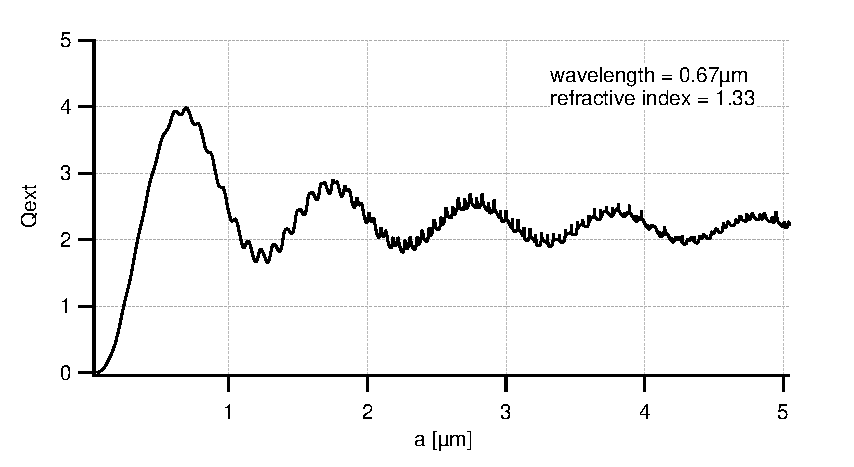
\includegraphics[width=16cm]{Qext_cloud.eps}
  \caption{雲粒の消散効率のサイズ依存性}\label{fig:qext}
 \end{center}
\end{figure}

図\ref{fig:qext}の$Q_{ext}(a)$は、$a\approx0.67\,\rm \mu m$で最初の極大（$Q_{ext}\approx4$）をとったあと、約$1\,\rm \mu m$の周期でゆるやかに増減しながら（極大は$a\approx1.7,\ 2.8,\ 3.8\,\rm \mu m$、極小は$a\approx1.3,\ 2.3,\ 3.3\,\rm \mu m$）$2$に近づく。この大きな波打ちは、粒子内部を通る光と粒子のまわりを回折する光の干渉によるもので、これに細かな波打ち（ミー共鳴）が重なっている。細かな波打ちは、雲粒の大きさのわずかなばらつきによって平均されてしまい、$\mathcal{T}(t)$にはほとんど現れない。

雲チェンバーの中で雲粒が成長するとき、1個の雲粒の消散断面積$\pi a^{2}Q_{ext}$は、$Q_{ext}$が極大を過ぎて減っていく区間で増え方が一時的に鈍る。このため光透過率$\mathcal{T}(t)$には、減少が一時的に止まる「こぶ（肩）」が、$a\approx1.0,\ 2.1,\ 3.1\,\rm \mu m$付近で順に現れる。逆に、$Q_{ext}$が極大に向かって増える区間（$a\approx0.5,\ 1.5,\ 2.5\,\rm \mu m$付近）では、$\mathcal{T}(t)$が急に下がる。このうち$a\approx1.0\,\rm \mu m$のこぶはごく浅い（モデルでは$\mathcal{T}$の変化が$0.5\%$程度）。はっきり見えるのは、$a\approx2\,\rm \mu m$のこぶ（$\mathcal{T}\approx0.95$、雲ができ始めてから約$0.3$秒後）と、$a\approx3\,\rm \mu m$のこぶ（$\mathcal{T}\approx0.90$、約$0.7$〜$0.9$秒後）である。以下では、これらを最初のこぶ、2つ目のこぶとよぶ。最初のこぶまでの$\mathcal{T}(t)$の形は主に雲粒の数で決まり、2つ目のこぶの時刻と深さには、雲粒の成長の速さ（水蒸気量）と光路長の情報が加わる。一方、時間がたつほど、$\mathcal{T}(t)$は雲粒の沈降や壁の影響を受けやすくなる。そこで本演習では、雲ができ始めてから2つ目のこぶまでの$\mathcal{T}(t)$の形を解析に用いる（\ref{sec:sbi}節）。

\clearpage




\section{雲チェンバーのしくみ}
本演習で用いる雲チェンバーの概略図を示す。


\begin{figure}[h]
 \begin{center}
  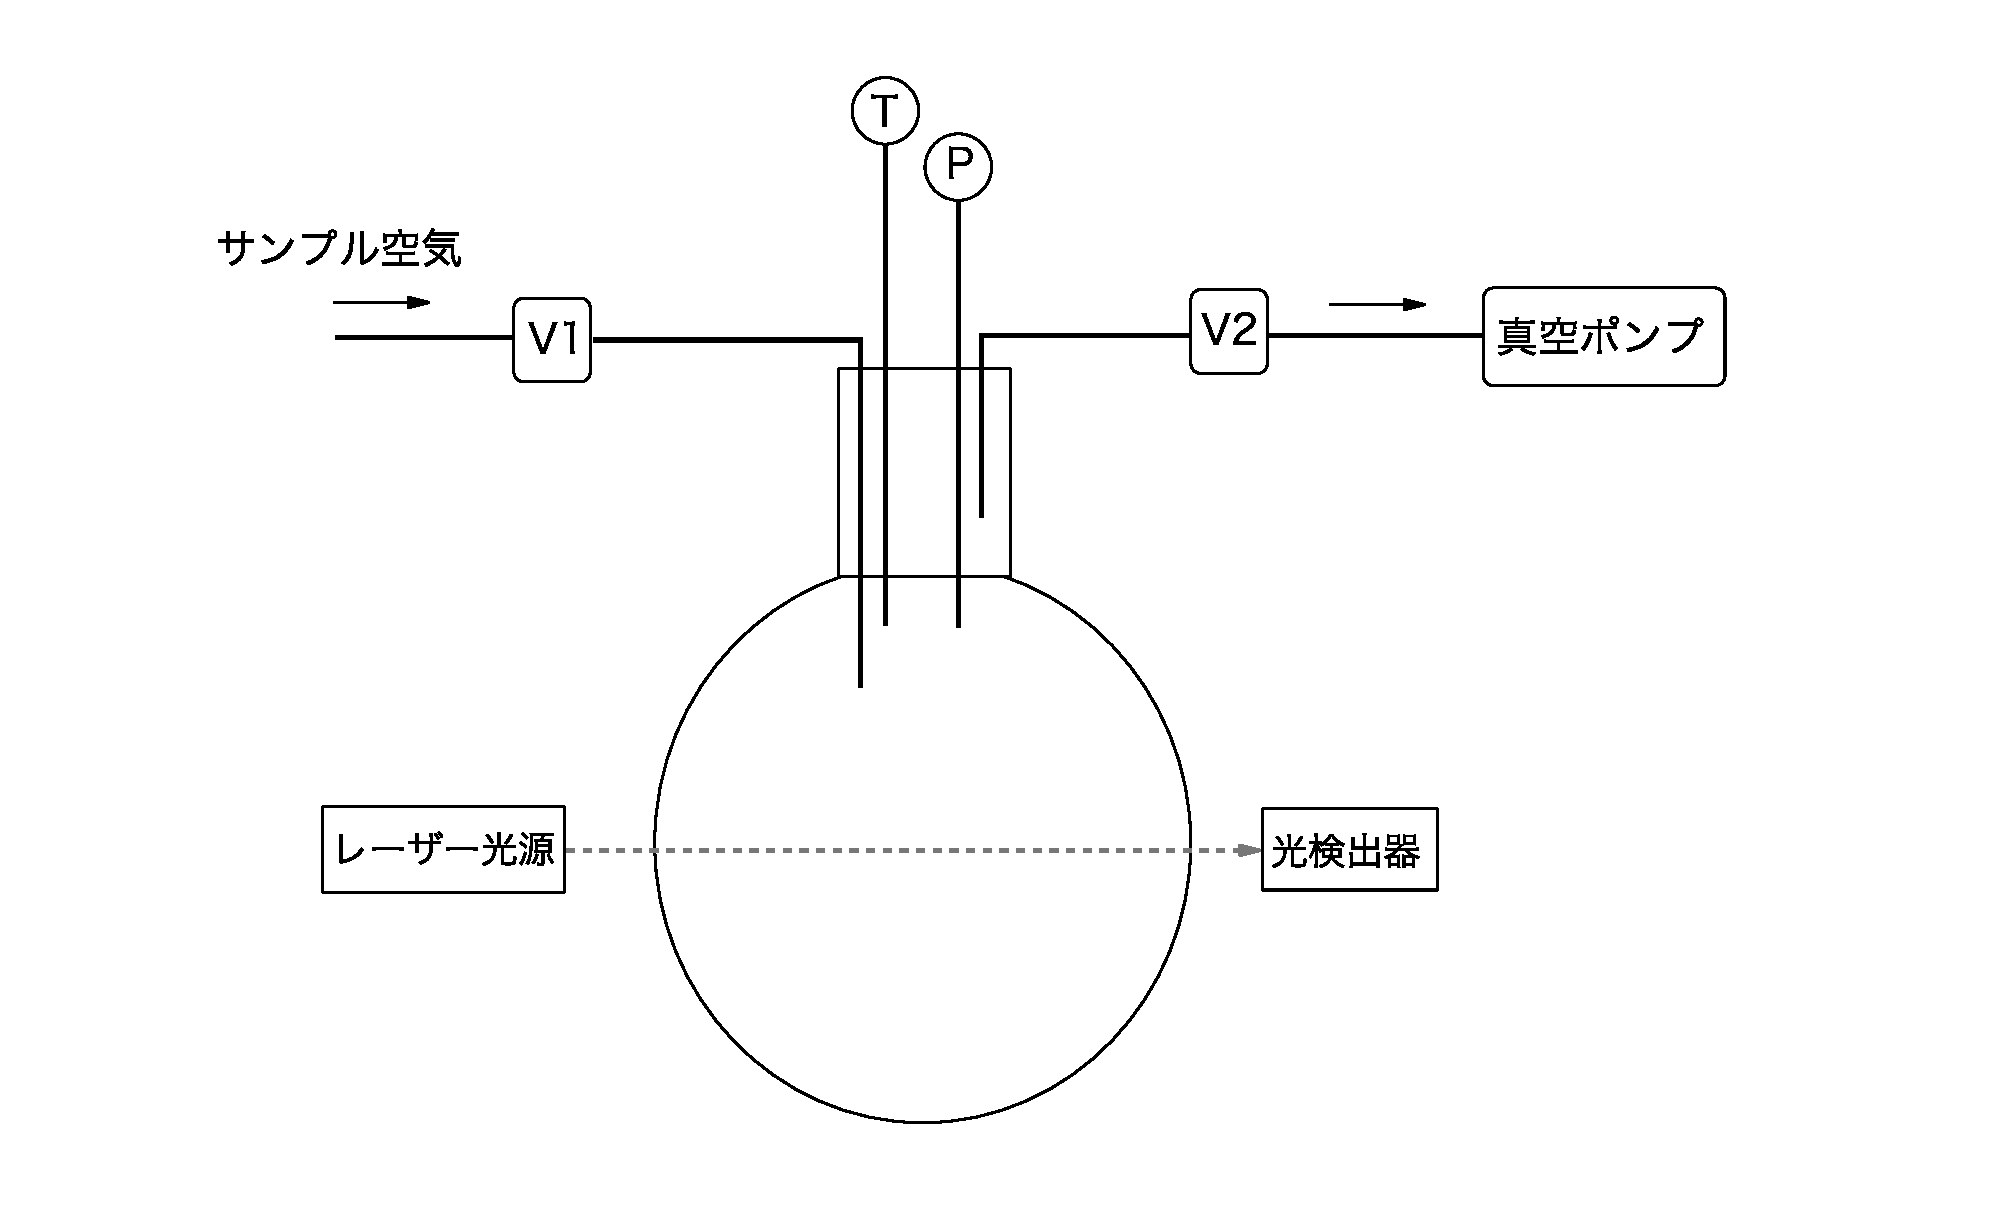
\includegraphics[width=16cm]{Chamber.eps}
  \caption{人工雲発生装置: $T, P, V$はそれぞれ温度センサー，気圧センサー，バルブを表す．}\label{fig:chamber}
 \end{center}
\end{figure}


この雲チェンバーでは、バルブV1、V2を共に開けて試料空気を導入したのち、V1,V2を共に閉じて空気を密閉する。その試料空気の初期温度$T_{ini}$と初期気圧$p_{ini}$を記録した後、V2を開けてチェンバー内の試料空気を減圧する。減圧開始から数秒間、圧力$p$と光透過率$\mathcal{T}$を10ミリ秒の時間分解能で測定する。　本節では、雲チェンバーの仕組みと製作について説明する。

センサーの電圧信号の取り込みとバルブの制御には、USBで接続するデータ収集装置（DAQ）NI USB-6210を用いる。USB-6210は16ビットのアナログ-デジタル変換器(ADC)を備え、アナログ入力ごとに入力電圧範囲を$\pm10,\,\pm5,\,\pm1,\,\pm0.2\,\rm V$から選べる。表\ref{tab:channels}に、本装置の信号と入力端子の割り当てを示す\footnote{2025年度まではNI USB-6008（12ビット）を用いていた。USB-6008では、気圧の分解能が約$3\,\rm hPa$、温度の分解能が約$0.3\,\rm K$と粗かった。}。
\begin{table}[h]
 \begin{center}
 \caption{DAQ（NI USB-6210）の端子の割り当て。アナログ入力はすべてシングルエンド（RSE）で、センサー側のGNDはAI GNDに接続する。}\label{tab:channels}
 \begin{tabular}{lll}
 \toprule
 端子 & 信号 & 入力電圧範囲 \\
 \midrule
 AI 0 & フォトダイオードの電流-電圧変換回路の出力 & $\pm10\,\rm V$ \\
 AI 1 & 気圧計の出力 & $\pm5\,\rm V$ \\
 AI 2 & サーミスタ回路の出力 & $\pm5\,\rm V$ \\
 AI 3 & 鏡面式露点計の相対湿度出力 & $\pm1\,\rm V$ \\
 AI 4 & 鏡面式露点計の露点温度出力 & $\pm1\,\rm V$ \\
 P1.0 (PFI 4) & バルブV1の駆動回路への信号 & デジタル出力 \\
 P1.1 (PFI 5) & バルブV2の駆動回路への信号 & デジタル出力 \\
 \bottomrule
 \end{tabular}
 \end{center}
\end{table}


\subsection{光検出機構}
雲チェンバーを通過する光線の放射束密度$I(t)$を測定できるようにするため、光検出器から出力される生の電流を、適切な電圧信号に変換してからコンピュータに取り込むための機構を製作する。本演習では、レーザー光源として赤色ダイオードレーザー(波長 670~nm, パワー $\sim$3 mW)を用い、光センサーとしてSi-フォトダイオード (感度 $\rm{\sim0.3\,A/W \, @ \,670\,nm}$)を用いる。Si-フォトダイオードは光電面へ入射する放射パワー[W]に比例した電流[A]を出力する\footnote{ここで用いるレーザー光線は単一方向への直進ビームであるため、光センサで測定される放射パワー$P\,\rm [W]$と、光線の放射束密度$I\,\rm [W\,m{-2}]$は比例する。このため、$\mathcal{T}(t) \equiv I(t)/I_{ref}= P(t)/P_{ref}$となる。}。Si-フォトダイオードから出力される微弱電流を、都合の良い大きさの電圧値に変換するために、オペアンプを用いた電流-電圧変換回路を用いる。

\begin{figure}[h]
 \begin{center}
  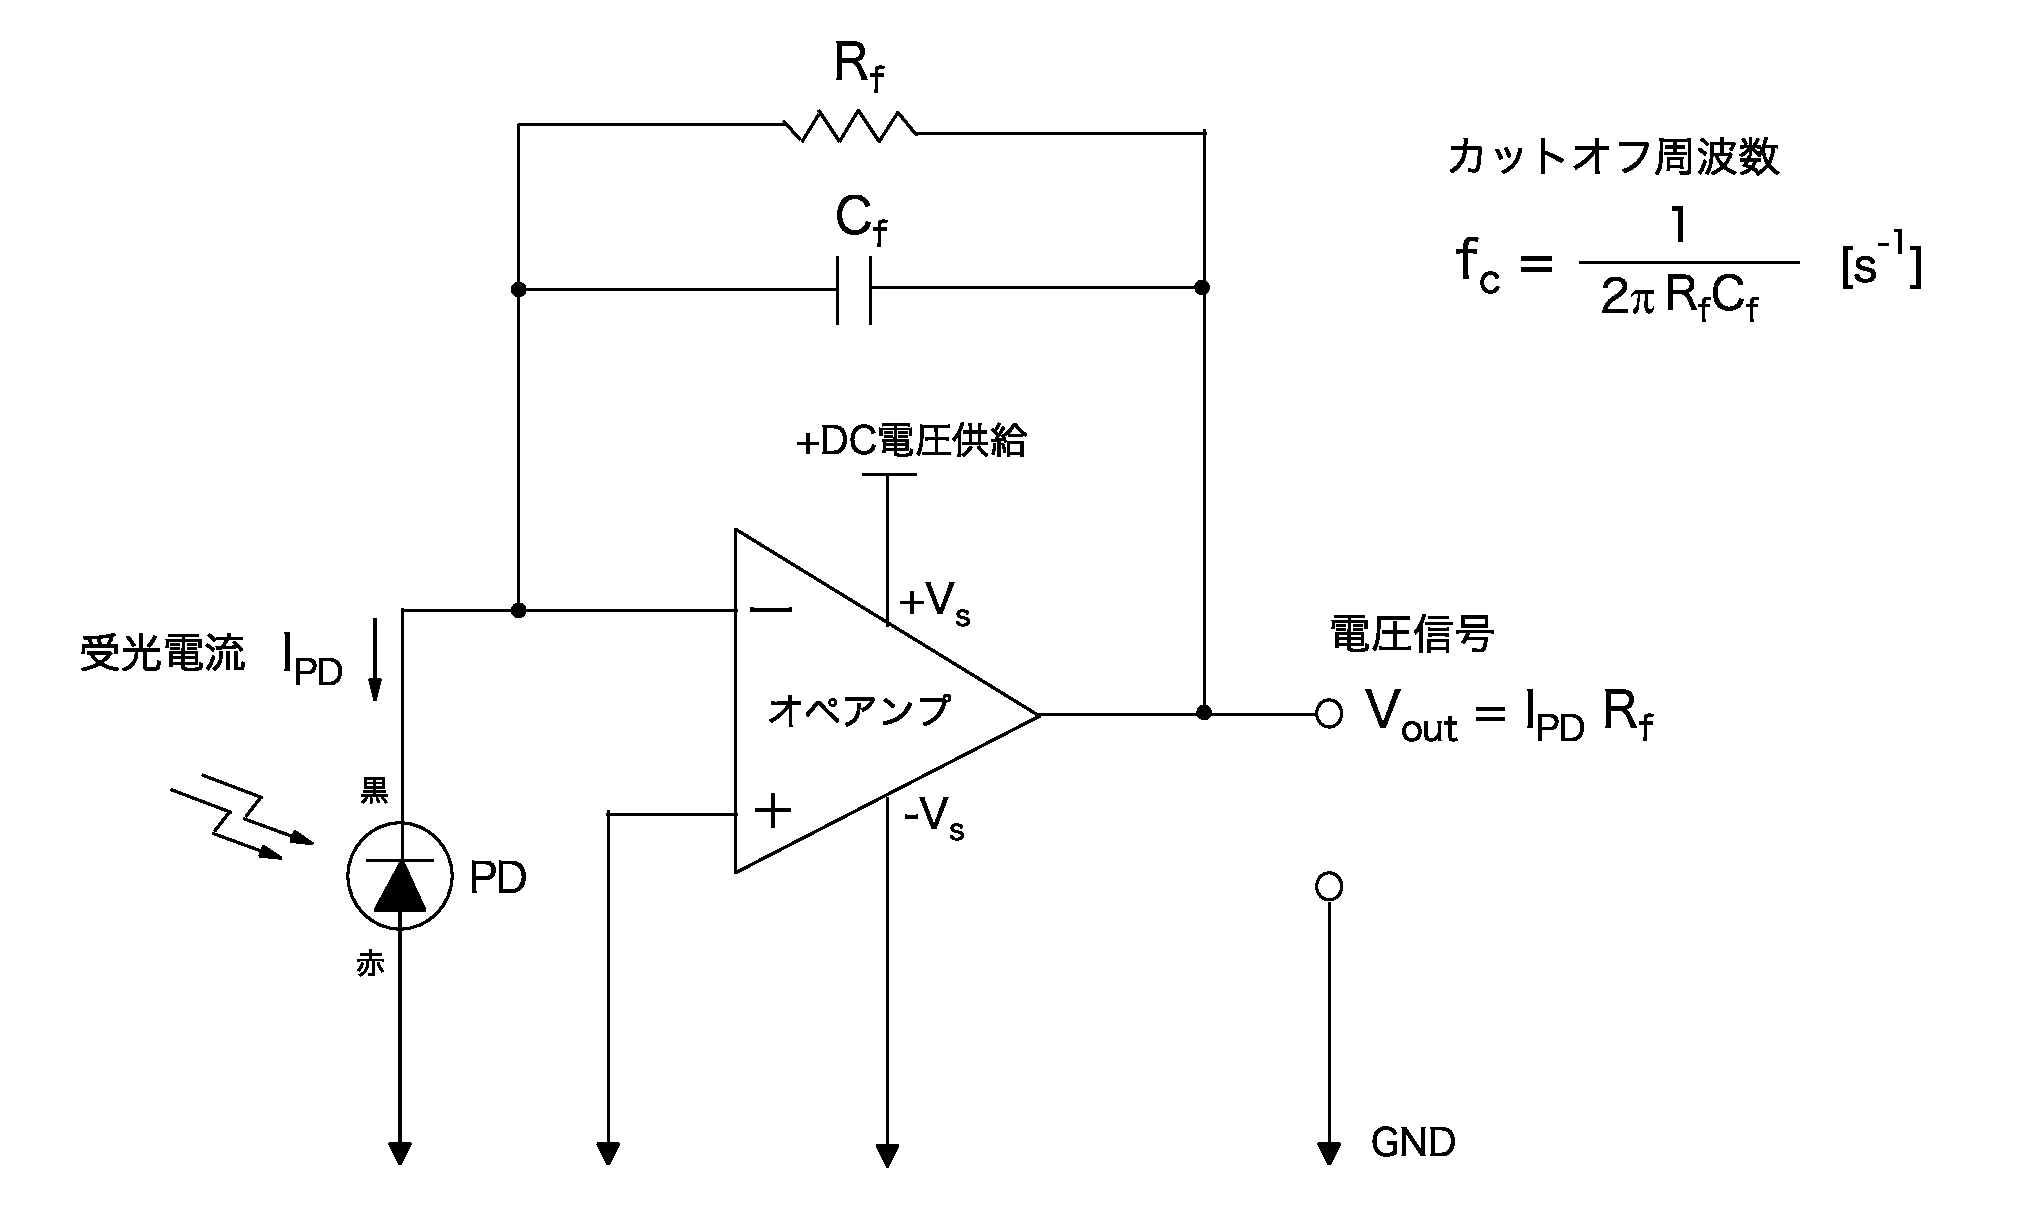
\includegraphics[width=12cm]{PD_circuit.eps}
  \caption{フォトダイオードの電流−電圧変換回路}\label{fig:pd}
 \end{center}
\end{figure}

入射する光の放射パワーの範囲に対応する電圧信号$V_{out}$の範囲が、ADCの入力電圧範囲を超えないように$R_{f}$の値を選ぶ。フォトダイオードの信号を取り込むADCの入力電圧範囲は $-10 \sim 10 \rm V $である。想定される$V_{out}$の最大値がADCの最大入力電圧の$0.5 \sim 0.8$倍くらいになるように設計するとよい。この電流-電圧変換回路は信号の高周波成分を除去するフィルターもかねている。コンデンサの容量$C_{f}$の値は、フィルターのカットオフ周波数$f_{c}$が適切な値となるように選ぶ。
\\
\begin{itembox}[l]{\bf{実習1. 光検出の電子回路の製作}}
\begin{enumerate}
\item Si-フォトダイオードへの入射光強度とADCの入力電圧範囲を考慮し、図3の回路における適切な$R_{f}$の値を決めなさい。その$R_{f}$において$C_{f}=0.1 \mu \rm F$としたとき、カットオフ周波数$f_{c}\, \rm [Hz]$はどうなるか？
\item ユニバーサル基盤上に図3の回路を実装しなさい。GNDは回路内の電位の基準点なので、回路内のすべてのGND端子は同じ電位でなければならない。基盤外への導線の長さは 0.5 m くらいにすること。
\item Si-フォトダイオードに光を当てた場合の出力電圧値$V_{out}$をデジタルマルチメーターで測定し、回路の動作を確認すること。
\end{enumerate}
\end{itembox}


\subsection{温度の測定}
温度測定センサーは多くの種類があるが、常温付近(-50℃〜100℃ 程度)の測定では、使い方が簡単で安価なサーミスタが使われることが多い。サーミスタは常温付近の温度変化に対する抵抗値変化がとても大きくなるように設計された特殊な抵抗体である。本演習では、温度上昇とともに抵抗値が減少するNTC(negative temperature coefficient)サーミスタを用いる。サーミスタ抵抗値の温度依存性は
\begin{equation}\label{eq:108}
 R=R_{0}\exp{{\bigg [}B{\bigg (}\frac{1}{T}-\frac{1}{T_{0}}{\bigg )}{\bigg ]}}
\end{equation}
という式で近似される。ここで$R_{0}$はあらかじめ基準温度$T_{0}$で計測された抵抗値であり、$R$は温度$T$における抵抗値である。本演習で用いるサーミスタの公称値は$T_{0}=298.15 \,\rm{K}$,\ $R_{0}=10 \,\rm{k}\Omega \pm1\%,\ B=3435 \,\rm{K}\pm1\% $ である\footnote{2025年度までの資料では、別の型番（NXFT15XH103FA2B）の値$B=3380\,\rm K$を記載していた。}。 また、このようなサーミスタのデータシートには、常温付近における温度検知用動作電流が 0.12 mA 程度と書かれている。この温度検知用動作電流は、サーミスタ自身の発熱による温度上昇が0.1℃となる電流と定義されている。サーミスタを流れる電流がこれよりも大きいとサーミスタ自身によるジュール熱の影響が無視できない可能性があるので、この程度の電流で動作させることが望ましい。

サーミスタの抵抗値を電圧信号として読み取るには、図\ref{fig:thermistor}に示した回路を用いる。図\ref{fig:thermistor}では、図\ref{fig:pd}には示していなかった電圧信号$V_{out}$の出力端子間(すなわちADCの電圧入力端子間)の抵抗$R_{in}$も表示している。その理由は、オペアンプを用いた図\ref{fig:pd}の回路では出力インピーダンスが数$\Omega$程度であり、$R_{in}$に比べて無視できるほど小さいために$R_{in}$は$V_{out}$の値に影響しないが、図\ref{fig:thermistor}の回路では、出力インピーダンス$R_{TH}$が$R_{in}$に比べて無視できるほど小さくはないため、$R_{in}$が$V_{out}$の値に影響するためである。本演習で用いるADC (NI USB-6210)では$R_{in}>10\, \rm{G}\Omega$であり、$R_{in}=\infty$とみなしてよい\footnote{以前用いていたNI USB-6008では$R_{in}=1.75\, \rm{M}\Omega$であり、$R_{in}$を無視すると温度が約$0.15\,\rm K$ずれる。}。本装置の回路では$V_{in}=5.07\,\rm V$、$R_{1}=29.5\,\rm k\Omega$である。

\begin{figure}[h]
 \begin{center}
  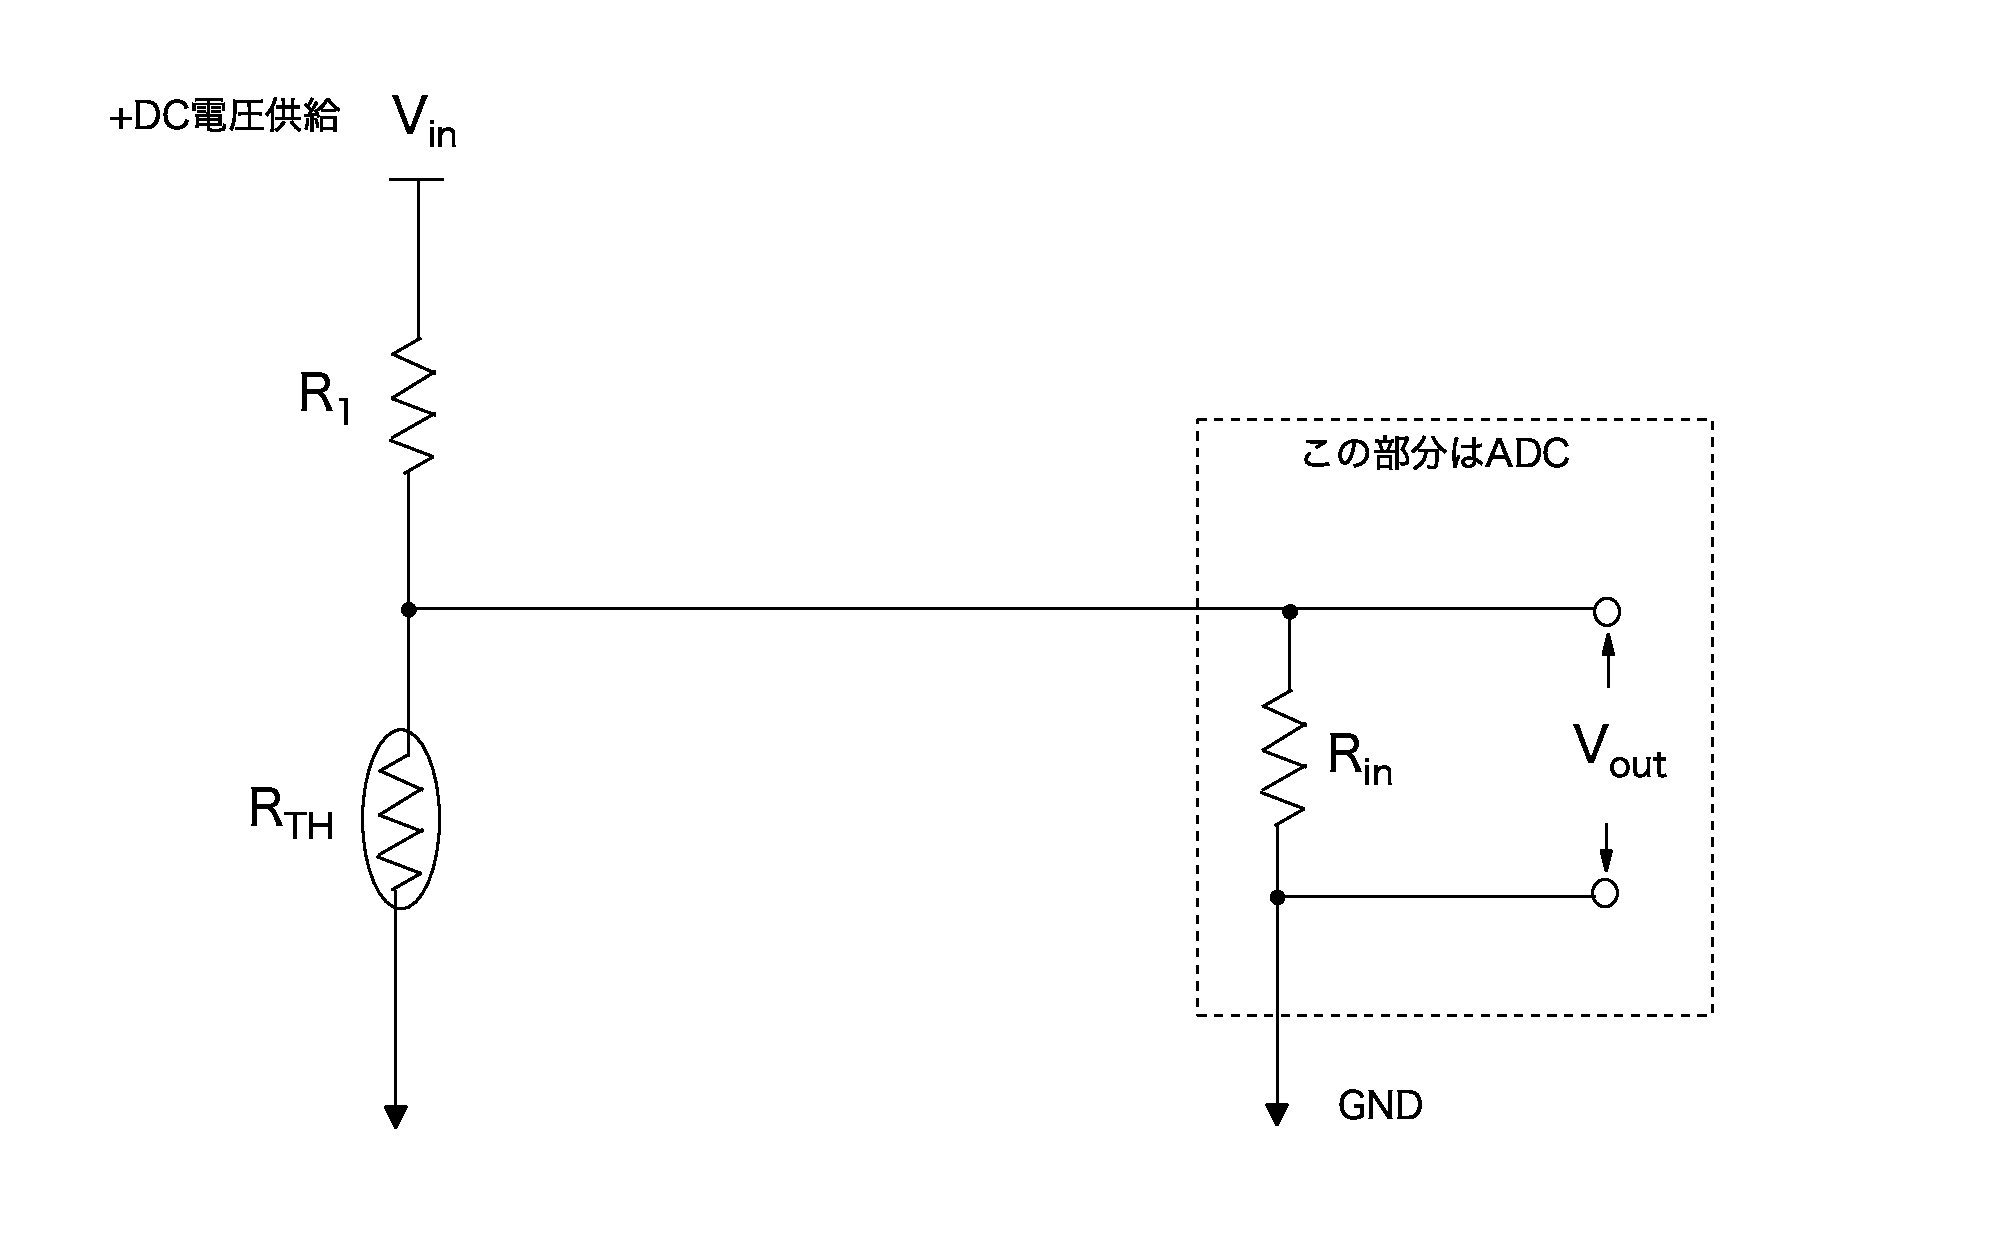
\includegraphics[width=14cm]{Thermister.eps}
  \caption{サーミスタの抵抗値$\rm{R_{TH}}$を電圧信号$\rm{V_{out}}$として読み出す回路}\label{fig:thermistor}
 \end{center}
\end{figure}

\paragraph{サーミスタの校正}
サーミスタの$R_{0}$には個体差（$\pm1\%$）があり、さらに配線の抵抗や回路の抵抗値の誤差も、実効的には$R_{0}$のずれとして現れる。$R_{0}$が$1\%$ずれると、温度は約$T^{2}/B\times0.01\approx0.26\,\rm K$ずれる。そこで、信頼できる温度計（本装置では鏡面式露点計に付属の温度計）の読み$T_{ref}$と、同時に測った$V_{out}$から、式\eqref{eq:108}と回路の式を$R_{0}$について解いて$R_{0}$を決める（１点校正）。$R_{in}$を含めると
\begin{equation}\label{eq:r0calib}
R_{0}=\frac{\exp{\big [}B{\big (}\frac{1}{T_{0}}-\frac{1}{T_{ref}}{\big )}{\big ]}}{\dfrac{1}{R_{1}}{\Big (}\dfrac{V_{in}}{V_{out}}-1{\Big )}-\dfrac{1}{R_{in}}}
\end{equation}
である。本装置では、公称値$R_{0}=10\,\rm k\Omega$のままでは温度が約$2\,\rm K$高く出ていたため、校正により$R_{0}=9.2\,\rm k\Omega$とした（2026年10月）。
\leavevmode \\
\begin{itembox}[l]{\bf{温度測定回路の作成 (今回は省略)}}
\begin{enumerate}
\item 図\ref{fig:thermistor}の回路における$V_{out}$を、$V_{in},R_{1},R_{TH},R_{in}$の関数として表しなさい。
\item 1.の結果と式\eqref{eq:108}を用いて、温度$T$を電圧信号$V_{out}$から計算するための式を導出しなさい。また、それを$R_{0}$について解いて式\eqref{eq:r0calib}を確かめなさい。
\item 図\ref{fig:thermistor}の回路において、$\rm{V_{in}} = 5 \rm{V}$の設定でサーミスタを使用するとき、このサーミスタの動作電流が適切な値になるように抵抗$R_{1}$の値を決めなさい。概算で十分なので、この計算では$R_{in}=\infty$と仮定してよい。
\item ユニバーサル基盤上に図\ref{fig:thermistor}のサーミスタ用回路を実装しなさい。回路外部へ接続される導線の長さは 0.5 m くらいでよい．
\item 室内空気中に置かれたサーミスタについて$V_{out}$を計測し、その$V_{out}$を2.の数式に代入して算出される温度$T$が正しいかどうか、信頼できる温度計と比較して確認しなさい。ずれていれば、式\eqref{eq:r0calib}で$R_{0}$を校正しなさい（配布コード\verb|calib_thermistor.py|）。
\end{enumerate}
\end{itembox}

\subsection{圧力の測定}\label{sec:pressure}
本演習では、圧力$p(t)$の測定のために、Setra社製のmodel 276気圧計を用いる。この気圧計は12 VDCの電源供給が必要で、$0\sim1380$ hPaの範
囲の気圧を、$0.1\sim5.1$ VDCの電圧信号として出力する。気圧と電圧の関係は一次式(線形)であり、$p\,[{\rm hPa}]=-27.6+276\,V_{out}\,[{\rm V}]$である。

減圧中の気圧は1秒間に数百hPaも変わるので、気圧計の読みがフラスコ内の気圧に遅れずについてくるとは限らない。実測の$\mathcal{T}(t)$を露点計の水蒸気混合比を与えたシミュレーションと比べると、本装置では、気圧計の読みはフラスコ内の気圧より約0.28秒遅れ、読みから求めた気圧の下がり幅は実際より約8\%大きいとすると、よく説明できる\footnote{記録した12サイクルで水蒸気混合比を露点計の値に固定して求め、別の12サイクルで検証した（水蒸気混合比を自由にして推定すると、露点計の値との差は$\pm6\%$以内）。気圧計までの配管の長さや取り付け位置によって変わりうるので、装置を組み替えたときは確かめ直す必要がある。}。この補正は\ref{sec:sbi}節の推定で用いる。\\
\begin{itembox}[l]{\bf{気圧センサーの使用 (今回は省略)}}
\begin{enumerate}
\item 気圧計に12 VDCを供給するための配線と、電圧信号を取り出すための配線を作りなさい。
\item 部屋の気圧における気圧センサーの出力電圧をデジタルマルチメータで測定し、部屋の気圧が何 hPaか確認しなさい。
\end{enumerate}
\end{itembox}

\subsection{バルブ制御機構}
ここでは、雲チェンバーの試料空気の置換や減圧操作を正確な再現性で繰り返し行えるようにするため、コンピュータからバルブを制御するための機構を製作する。本演習では、大流量の空気が流れる配管の開閉制御のために使用できる、電動ボールバルブ\footnote{開状態において配管内の障害構造物がないため、流体抵抗が小さい。}を用いる。本演習では電動ボールバルブとしてKITZ社製ED24-UTE（駆動電源電圧24VDC）を用いる、電動ボールバルブを制御するために、リレーとトランジスタを用いた駆動回路を用いる(図\ref{fig:relay})。この回路では、まずコンピュータからのデジタル電圧信号をDAQのデジタル出力端子（表\ref{tab:channels}）から出力し、その電圧値を微弱な電流値に変換し、その微弱な電流値をトランジスタで増幅したのち、その電流をリレーの制御端子に入力している。トランジスタで電流を増幅する理由は、DAQのデジタル信号端子から出力される電流はとても小さく、リレーを直接駆動するには十分でないためである。本演習では、回路を単純化するため、電動ボールバルブと同じ駆動電圧（+24VDC）のリレーを用いる。


\begin{figure}[h]
 \begin{center}
 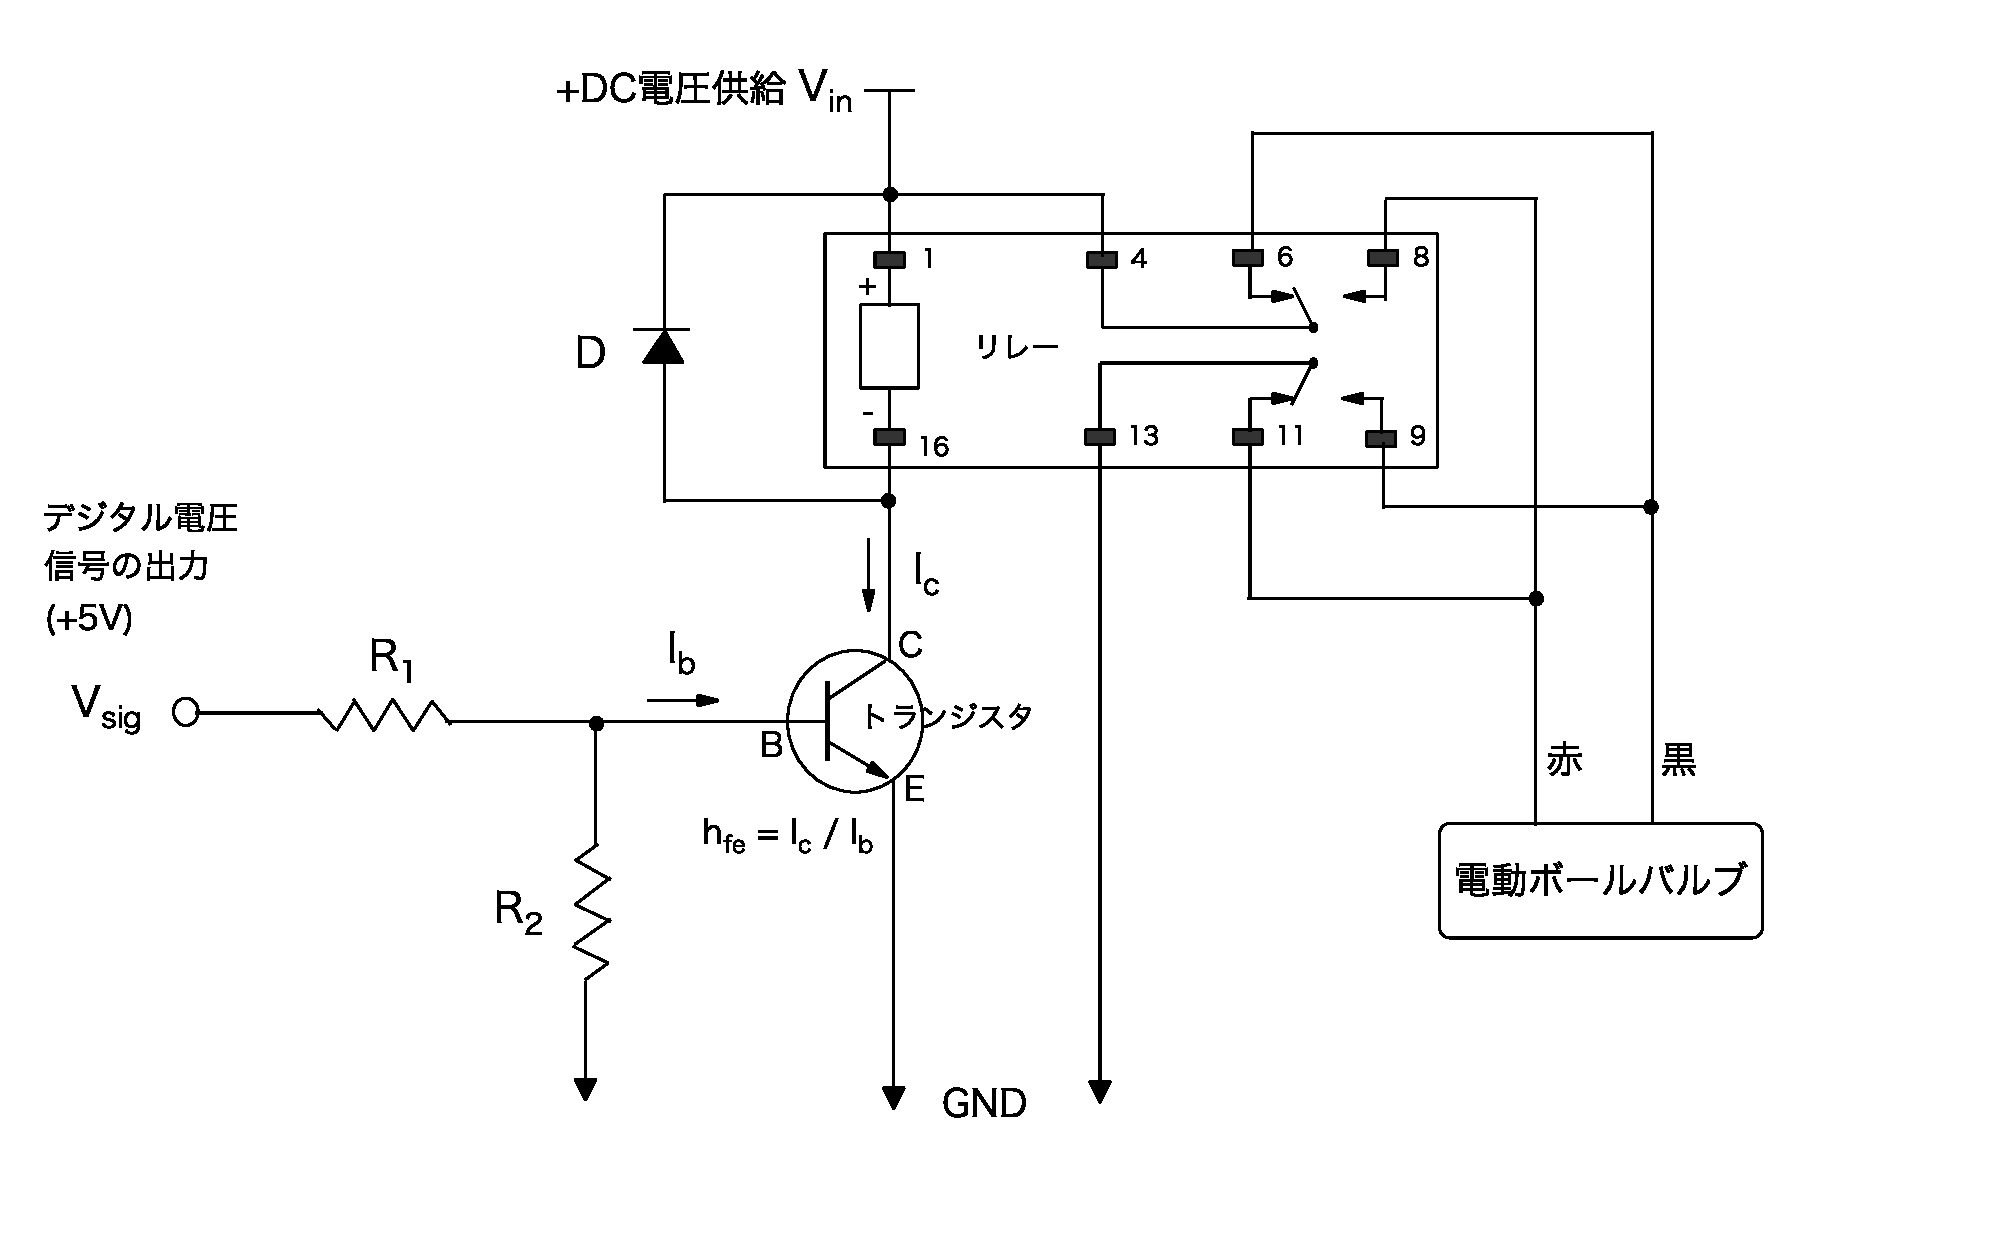
\includegraphics[width=18cm]{Relay_circuit.eps}
  \caption{トランジスタとリレーを用いた電動ボールバルブの駆動回路}\label{fig:relay}
 \end{center}
\end{figure}


図\ref{fig:relay}において、$V_{sig}$はデジタル信号電圧（ここでは+5VDC）、$V_{in}$はリレーと電動ボールバルブの動作電圧(ここでは+24VDC)、$I_{b}$はベース電流、$I_{c}$はコレクタ電流、$h_{fe}$はトランジスタの電流増幅率$(=I_{c}/I_{b})$、$D$は電流OFF時に発生する逆電圧スパイクを吸収するための整流用ダイオードである。本演習で用いるトランジスタ(東芝 2SC1815Y)は、$h_{fe}=120 \sim 240$という増幅率を持っている。リレーを安定に動作させるには$I_{c}$がリレーの定格電流$I_{relay}$（リレーのデータシートに記載）の$\sim3$倍であることが望ましい。増幅後の$I_{c}$の値がそうなるように$I_{b}$の値を設定する。この回路において$I_{b}$を決めているのは$R_{1}$である。$R_{2}$はトランジスタの誤動作防止のため（OFF時のベース電圧をGNDに保つため）につけるもので、$I_{b}$にはほとんど影響しない。通常、$R_{2}$は$R_{1}$の$2 \sim 10$倍程度に設定する。このトランジスタのベース-エミッタ間の電圧$V_{be}$は常に0.65V程度である。これらを踏まえると、
\begin{equation}\label{eq:109}
 I_{c} = K I_{relay},\ ただし\  K\sim3.
\end{equation}
となるように $R_{1}$の値を
\begin{equation}\label{eq:110}
 R_{1}=\frac{V_{sig}-V_{be}}{I_{b}}=\frac{(V_{sig}-V_{be})h_{fe}}{I_{c}}
\end{equation}
となるように選べばよい。ここで、増幅率$h_{fe}$としては最低値である120を仮定する。

本演習で使用するリレー(OMRON社製 G6A-274P-ST-US DC24V)は、動作電圧 $V_{in}=24 \,\rm{VDC}$, 定格電流 $I_{relay}=8.3 \,\rm{mA}$である．
\\
\begin{itembox}[l]{\bf{実習2. バルブ駆動回路の製作}}
\begin{enumerate}
\item 図\ref{fig:relay}の電動ボールバルブ駆動回路における$R_{1},R_{2}$の値を決めた上で、この回路をユニバーサル基盤上に実装しなさい。
\item デジタル電圧信号$V_{sig}$のON/OFFで電動ボールバルブを開閉できることを確認しなさい。DAQのデジタル出力の電圧（Highのとき）をデジタルマルチメーターで測り、$V_{sig}$の想定（+5 V）と合っているかも確かめること。
\end{enumerate}
\end{itembox}
\\
\subsection{参照測定器}\label{sec:reference}
雲チェンバーによる推定値を検証するため、市販の測定器でも同じ空気を測る。
\paragraph{鏡面式露点計}
鏡面式露点計（東京光電子工業 DPH-203B）は、空気に触れる小さな鏡を電子冷却で冷やし、鏡に露がつき始める温度、すなわち露点温度$T_{d}$を光学的に検出する。測定原理が露点温度の定義そのものなので、正確である。DPH-203Bは露点温度を電圧（約$10\,\rm mV/℃$）で、相対湿度を電圧（$0\sim1\,\rm V$が$0\sim100\%$）で出力する。露点温度は、５点の校正データに直線をあてはめた式
\begin{equation}\label{eq:td_calib}
T_{d}\,[℃]=0.100574\times V\,[{\rm mV}]-0.1018
\end{equation}
で換算する（残差の二乗平均$0.06\,℃$）\footnote{DPH-203Bの取扱説明書には「4〜20 mAの電流出力」と書かれているが誤りで、実際は電圧出力である。}。露点温度$T_{d}$と気圧$p$から、水蒸気圧$e$と水蒸気混合比$q_{v}$を、マグヌス式（WMO, 2018）
\begin{equation}\label{eq:magnus}
e=611.2\exp{\bigg (}\frac{17.62\,T_{d}}{243.12+T_{d}}{\bigg )}\ [{\rm Pa}],\ \ \ q_{v}=\frac{\varepsilon e}{p-e}
\end{equation}
で求める（$T_{d}$の単位は℃、$\varepsilon=0.622$）。マグヌス式は、\ref{sec:clausius}節で導くクラウジウス-クラペイロンの式を、実測の平衡水蒸気圧によく合うように修正した経験式である。外気の露点温度が室温より高いときは、配管やチェンバーの壁で結露して試料空気の水蒸気が減ってしまうので、配管と測定器を外気の露点温度より高い温度に保つ必要がある。
\paragraph{凝縮粒子計数器（CPC）}
凝縮粒子計数器（condensation particle counter, CPC）は、試料空気をアルコールなどの過飽和蒸気の中に通して、小さな粒子を光学的に検出できる大きさまで成長させ、１個ずつ数える。本演習では、TSI社製 model 3022Aを用いる。このCPCはブタノールの蒸気を用い、直径約7 nm以上の粒子を数える（データシートを参照のこと）。CPCは雲チェンバーよりはるかに高い過飽和度で粒子を成長させるので、雲チェンバーでは活性化しない小さな粒子も数える。CPCの値は、RS-232（USB-シリアル変換）で計測制御のソフトウェアが1秒ごとに読み取り、雲チェンバーのデータと同じPCの時計で記録する。CPCは雲チェンバーと同じ試料配管から吸引しているので、バルブV1が開いて配管の空気が動く間の数秒間は、CPCの値が大きく下がる。そこで、各サイクルの記録には、配管が静止している間（V1が閉じている密閉の最後の3秒から減圧の終わりまで）の中央値を用いる。
\\
\subsection{計測制御のソフトウェア}\label{sec:software}
本節では、バルブ開閉を制御し光透過率と圧力の時系列データを記録・解析するためのソフトウェア\footnote{Pythonで開発している（配布コードのフォルダ\texttt{cloudchamber}）。使い方の詳細は操作マニュアル\texttt{MANUAL.md}を参照のこと。2025年度まではLabVIEWで開発したソフトウェアを用いていた。}の機能を説明する。ソフトウェアには、以下の制御サイクルを自動で繰り返す「自動運転」と、画面のボタンでバルブを１つずつ開閉する「手動運転」がある（手動運転ではデータを記録しない）。自動運転中のバルブ開閉状態の動作とその実行順序は以下のとおりである。
\begin{itembox}[l]{バルブの制御サイクル}
\begin{enumerate}
\item 空気置換: V1, V2ともに開状態とし、古い空気を追い出しつつ新たな試料空気を雲チェンバーに取り込む。このとき流れる空気の摩擦抵抗により、雲チェンバー内の圧力は外圧よりも少し低くなる。
\item 気圧緩和: V1を開状態, V2を閉状態とし、排気を止めることで雲チェンバー内の圧力を外圧になじませる。
\item 密閉: V1を閉状態, V2を閉状態とし、試料空気をチェンバー内に閉じ込める。この段階の終わりに、基準光強度$I_{ref}$（直近10秒の中央値）、初期圧力$p_{ini}$と初期温度$T_{ini}$（直近1秒の中央値）、露点計の露点温度と相対湿度（直近10秒の中央値）を確定する。
\item 減圧: V1を閉状態, V2を開状態とし、排気により試料空気を減圧する。このとき、圧力と光透過率の時間プロファイルを測定する。
\item 開放: V1を開状態, V2を閉状態とし、減圧状態から常圧に戻す。この間に、直前の減圧のデータを解析し、水蒸気混合比とエアロゾル数濃度を推定する。
\item 待機: V1を開状態, V2を閉状態としたまま待つ。バルブ制御１サイクルの長さを調節するための動作。
\end{enumerate}
\end{itembox}
ソフトウェア実行前に各動作の継続時間をソフトウェアの設定欄に入力しておく（既定値は各10秒で、１サイクル60秒）。実行中は動作$1 \sim 6$からなる制御サイクルをずっと繰り返す。アナログ入力は、DAQのハードウェアクロックにより100 Hz（10ミリ秒ごと）で取り込む。

減圧の段階では、V2を開ける指令を出してから実際に気圧が下がり始めるまでに、バルブの動作による遅れがある。そこで、気圧が実際に下がり始めた時刻$t_{0}$をフィットで求め、以下では$t_{0}$を時刻の原点$t=0$とする。本演習で用いる雲チェンバーでは、減圧時の圧力の時間プロファイル$p(t)$はおおまかには以下の関数で近似される。
\begin{equation}\label{eq:111}
 p(t)\approx {\big (}p_{ini}-p_{\rm offset}{\big )} {\rm exp}{\bigg (}- \frac{t}{\tau_{\rm vac}} {\bigg )}+ p_{\rm offset}
\end{equation}
しかし、実測の$p(t)$を詳しく見ると、式\eqref{eq:111}は減圧初期の曲線をよく再現しない（残差の二乗平均が約4 hPa）。その原因は２つある。１つは、ボールバルブが全開になるまでに約0.6秒かかり、その間は排気の流れやすさ（コンダクタンス）が時間とともに大きくなることである。もう１つは、チェンバーと配管の容積や流れ方の違いにより、速く減る成分とゆっくり減る成分があることである。そこで、バルブが開く時間$t_{open}$の間はコンダクタンスが時間に比例して増えるとし、２つの指数関数の和で表した
\begin{equation}\label{eq:ramp2}
\begin{split}
&p(t)= p_{\rm offset}+ {\big (}p_{ini}-p_{\rm offset}{\big )}{\bigg [} f\exp{\bigg (}-\frac{G(t)}{\tau_{1}}{\bigg )}+(1-f)\exp{\bigg (}-\frac{G(t)}{\tau_{2}}{\bigg )}{\bigg ]},\\
&G(t)=\begin{cases} \dfrac{t^{2}}{2t_{open}} & (0\le t<t_{open}) \\[2mm] t-\dfrac{t_{open}}{2} & (t\ge t_{open}) \end{cases}
\end{split}
\end{equation}
を用いる（$f$は速い成分の割合）。式\eqref{eq:ramp2}では、減圧初期の残差の二乗平均は約1 hPaになる。典型的な値は$t_{open}\approx0.6\,\rm s$、$f\approx0.7$、$\tau_{1}\approx1.9\,\rm s$である\footnote{$p_{\rm offset}$と$\tau_{2}$は互いに相関が強く、別々には精度よく決まらない。しかし、雲ができる時刻までの$p(t)$はよく再現されるので、推定には差し支えない。}。シミュレーションでは、実測された生の$p(t)$データの代わりに、これらの近似関数で表現した$p(t)$を用いることにする。

バルブ制御１サイクル毎に画面に表示され、かつ１日ごとのファイル\verb|cloud_data_YYYYMMDD.csv|（YYYYMMDDは日付）の各行に記録される主な情報は下記のとおり\footnote{すべての列の説明は操作マニュアルを参照のこと。}。
\\
\begin{itembox}[l]{1サイクルごとの主な記録情報}
\begin{enumerate}
\item \verb|Time_stamp|, \verb|datetime|: 減圧の段階を始めた時刻（UNIX時刻と、現地時刻の文字列）。
\item \verb|T_ini|: 初期温度 [K]。
\item \verb|p_ini|: 初期圧力 [hPa]。
\item \verb|p_offset|, \verb|tau_vac|: 実測$p(t)$を関数\eqref{eq:111}でフィットしたときのパラメータ [hPa], [s]。
\item \verb|t0_ramp2|, \verb|p_offset2|, \verb|tau_vac1|, \verb|frac1|, \verb|tau_vac2|, \verb|t_open|, \verb|p_rms|: 実測$p(t)$を関数\eqref{eq:ramp2}でフィットしたときのパラメータ$t_{0}, p_{\rm offset}, \tau_{1}, f, \tau_{2}, t_{open}$と残差の二乗平均。
\item \verb|p_c|: 雲ができ始めたときの圧力 [hPa]。これは式\eqref{eq:117}中の$p(t=t_{c})$と同じ。
\item \verb|zeta_moist|, \verb|zeta_turbid|: 式\eqref{eq:117}, \eqref{eq:118}で定義される$\mathcal{T}(t)$の特徴量。
\item \verb|qw_gkg|, \verb|Td_est|, \verb|nd_cm3|: 推定した水蒸気混合比 [g/kg]、それに対応する露点温度 [℃]、エアロゾル（雲凝結核）数濃度 [個/cm$^{3}$]。それぞれに90\%信用区間の下限・上限（\verb|_lo|, \verb|_hi|）がつく（\ref{sec:sbi}節）。
\item \verb|ref_Td|, \verb|qw_ref_td_gkg|: 露点計の露点温度 [℃] と、それから式\eqref{eq:magnus}で求めた水蒸気混合比 [g/kg]。
\item \verb|flags|: 異常の印（雲ができなかった、など）。
\end{enumerate}
\end{itembox}
また、減圧ごとに、時刻$t$、気圧$p(t)$、光透過率$\mathcal{T}(t)$、温度の10ミリ秒ごとの生データを、フォルダ\verb|raw_YYYYMMDD|の中のファイル（NumPy形式）に保存する。生データがあれば、解析法を改良したあとで過去のデータを推定し直すことができる。


\section{シミュレーションとデータ解析}　
本節では、雲チェンバーの中での湿潤空気塊の内部変数と光透過率の時間発展のシミュレーション法（順問題モデル）と、光透過率の測定結果から湿潤空気塊の性質を推定するデータ解析法（逆問題モデル）について説明する。

\subsection{シミュレーション（順問題）のモデル}
装置のなかで起こっている現象をコンピュータを用いてシミュレーションする意義として、以下の３つが挙げられる。
\begin{enumerate}
\item 直接観察できない内部変数や変数間の相互作用について理解する手がかりが得られる。
\item 観測可能な変数のシミュレーション値と実測値との比較は、モデルの妥当性の判断材料となる。
\item 順問題を解くためのモデルは、逆問題を解くためにしばしば必要となる。
\end{enumerate}
本節では、1-3節で解説した事項をもとに、図\ref{fig:chamber}の雲チェンバーの中での雲粒成長とそれに伴うレーザー光線透過率の時間変化を予測するための方程式群と算法について解説する。 
単位質量の湿潤空気塊が含んでいる雲粒数を$n_{d}\,\rm [個\,kg^{-1}]$と定義する。また、断熱空気塊中の雲粒の凝縮成長における近似として、すべての雲粒について、各時刻で粒径は同一と仮定する。このとき、雲水混合比$q_{l}$は
\begin{equation}\label{eq:112}
 q_{l}=\frac{4 \pi}{3}\rho_{l} a^{3} n_{d}
\end{equation}
と表される。ところで、空気塊内の水の質量保存則により、水蒸気混合比$q_{v}$、雲水混合比$q_{l}$、総水混合比$q_{w}$との関係は、
\begin{equation}\label{eq:113}
 q_{v}=q_{w}-q_{l}
\end{equation}
となっている。式\eqref{eq:112},\eqref{eq:113}から、水蒸気混合比の時間微分は、雲粒半径とその成長速度により
\begin{equation}\label{eq:114}
 \frac{dq_{v}}{dt} =- 4 \pi n_{d} \rho_{l} a^{2} \frac{da}{dt}
\end{equation}
と表される。　

雲粒を含まないチェンバーを通過した光線の放射束密度を$I_{ref}$、雲粒を含むチェンバーを通過した光線の放射束密度を$I$とおくと、 チェンバーの光透過率$\mathcal{T}(t)$は、式\eqref{eq:104},\eqref{eq:106},\eqref{eq:107}から、
\begin{equation}\label{eq:115}
\mathcal{T}(t)= \frac{I(t)}{I_{ref}}=\exp {\bigg [}-\pi a^2(t) Q_{ext}(a(t)) \cdot \frac{p(t)}{R_{d}T(t)}n_{d} \cdot L {\bigg ]}
\end{equation}
と表せる。ここで光路長$L$は雲チェンバーの直径である。本演習で用いる小型の雲チェンバー（$L=0.2 \, \rm m$）では、エアロゾルによる光透過率の減少は無視できるほど小さい。そこで、減圧開始直前の数秒間における放射束密度$I(t)$の中央値を、式\eqref{eq:115}中の$I_{ref}$として採用することにする。

減圧時の$p(t)$の時間プロファイルと、減圧開始時の温度$T$が実測から分かっているとし、また雲粒半径$a$の初期値（=雲凝結核となるエアロゾル粒子の半径）を典型的な値（例えば$a=0.05 \mu m$）に仮定するものとする。このとき、水蒸気混合比$q_{w}$と単位質量当たりの雲凝結核数$n_{d}$を入力値として与えれば、以下のアルゴリズムにより、温度$T(t)$、水蒸気混合比$q_{v}(t)$、雲粒半径$a(t)$、レーザー光透過率$\mathcal{T}(t)$の時間発展をシミュレーションできる。
\\
\begin{itembox}[l]{アルゴリズム}
\begin{enumerate}
\item 減圧開始時刻$t=0$において、各パラメータに初期値を代入。
\item 経過時間$t$において、式\eqref{eq:115}により、$a, p, T, n_{d}$から光透過率$\mathcal{T}$を算出。
\item 経過時間$t$において、式\eqref{eq:112}により、$a, n_{d}$から雲水混合比$q_{l}$を算出。
\item 経過時間$t$において、式\eqref{eq:113}により、$q_{w}, q_{l}$から水蒸気混合比$q_{v}$を算出。
\item 経過時間$t$において、式\eqref{eq:17}により、$p, q_{v}$から水蒸気圧$e$を算出。
\item 経過時間$t$において、式\eqref{eq:21}により、$T, e$から飽和比$S$を算出。
\item 経過時間$t$において、式\eqref{eq:102}	により、$T_{\infty}(=T), S$から雲粒温度$T_{0}$を算出 （ニュートン法で求解）。
\item 経過時間$t$において、式\eqref{eq:103}により、$T_{\infty}(=T), T_{0}, a$から雲粒半径の時間微分$da/dt$を算出。
\item 経過時間$t$において、式\eqref{eq:114}により、$a, da/dt$から$dq_{v}/dt$を算出。
\item 経過時間$t$において、式\eqref{eq:71}により、$q_{v}, q_{l}$から湿潤空気塊の定圧比熱$c_{p}$を算出。
\item 経過時間$t$において、式\eqref{eq:74}により、$dq_{v}/dt, c_{p}, p, dp/dt$から$dT/dt$を算出。
\item $a(t), da/dt(t)$の現在値から、$a(t+\Delta t)$の値を算出。
\item $T(t), dT/dt(t)$の現在値から、$T(t+\Delta t)$の値を算出。
\item $t$の値を、$t+\Delta t$に更新\footnote{配布コードでは、タイムステップ幅は$\Delta t=1\times10^{-3}\rm s$ としている}。
\item 経過時間$t$が設定した上限値になるまで、2に戻ってくりかえし。
\end{enumerate}
\end{itembox}

このシミュレーション計算のための配布コード\verb|CloudChamberSimulator.py|では、まず、空気の初期温度$T_{ini}$と初期圧力$p_{ini}$、圧力$p(t)$の時間プロファイルのパラメータ$p_{\rm offset}, \tau_{\rm vac}$を、雲チェンバーを運転したときの代表値に設定しておく。入力値である水蒸気混合比$q_{w}(=q_{v})$と雲凝結核数濃度$n_{d}$を設定して実行すると、減圧開始から数秒間における変数群$(T,e,q_{v},S,a,\mathcal{T})$の時間プロファイルの計算結果がファイルに出力される。
\\
\begin{itembox}[l]{\bf{実習3. シミュレーションの実行}}
\begin{enumerate}
\item 雲凝結核数濃度$n_{d}$を典型値に固定しておき、水蒸気混合比$q_{w}(=q_{v})$の値を変えたとき飽和比$S(t)$、雲粒半径$a(t)$、光透過率$\mathcal{T}(t)$がどのように変わるか調べてみよう。結果の可視化のために、配布コード\verb|Load_and_Plot_CSVdata.py|を適宜修正して使ってよい。
\item 水蒸気混合比$q_{w}$を典型値に固定しておき、雲凝結核数濃度$n_{d}$の値を変えたとき飽和比$S(t)$、雲粒半径$a(t)$、光透過率$\mathcal{T}(t)$がどのように変わるか調べてみよう。
\end{enumerate}
\end{itembox}

\subsubsection{拡張モデル}\label{sec:extended}
上のモデルは、すべての雲粒が同じ大きさで、減圧開始時から雲粒として成長すると仮定している。実際には、雲チェンバーの中のエアロゾル粒子の大きさや成分はさまざまで、\ref{sec:activation}節で述べたように、飽和比$S$が各粒子の臨界飽和比$S_{c}$を超えた粒子だけが雲粒になる。また、雲粒ができ始めるまでの時間は、$p(t)$の減圧初期の形に敏感である。実測の$\mathcal{T}(t)$を定量的に解析するため、計測制御ソフトウェア（\verb|cloudchamber/activation.py|）では、上のモデルを以下のように拡張している。
\begin{enumerate}
\item エアロゾル粒子の乾燥半径の分布を対数正規分布（幾何平均半径$r_{g}$、幾何標準偏差$\sigma_{g}$）とし、これを個数の等しい12個の区間に分けて、区間ごとに水滴の半径$a_{j}(t)$の時間発展を解く。吸湿性は$\kappa$で表す。
\item 減圧開始時の水滴は、初期の飽和比（相対湿度）で平衡になったヘイズ粒子とする。成長速度は、溶質効果・曲率効果を含む式\eqref{eq:growth_general}と、補正した拡散率・熱伝導率\eqref{eq:kinetic}で計算する。$S<S_{c}$の小さなヘイズ粒子は、計算の時間ステップより短い時間で平衡に達するので、平衡半径（$S_{eq}(a)=S$の解）で置き換える。
\item 雲水混合比は$q_{l}=\frac{4\pi}{3}\rho_{l}\sum_{j}a_{j}^{3}n_{d}/12$、光透過率は$\mathcal{T}=\exp{\big [}-\sum_{j}\pi a_{j}^{2}Q_{ext}(a_{j})\,\rho\, n_{d} L/12{\big ]}$とする。$L$は光が雲の中を通る長さ（実効光路長、$0.18\,\rm m$）である。$Q_{ext}$は、同じ区間の中の雲粒の大きさのわずかなばらつきについて平均した値を用いる。拡散成長では$da/dt\propto1/a$なので、$a\,\delta a$が一定に保たれ、半径の相対的なばらつき$\delta a/a$は$a^{-2}$に比例して小さくなる。そこで、相対標準偏差を$\sigma(a)=\max\left[\sigma_{1}(a/0.69\,{\rm \mu m})^{-2},\ \sigma_{\rm floor}\right]$とする（$\sigma_{1}$は$Q_{ext}$の最初の極大$a=0.69\,\rm \mu m$でのばらつき、$\sigma_{\rm floor}$は活性化の時刻の違いなどで残るばらつき）。
\item 圧力$p(t)$は式\eqref{eq:ramp2}で与え、式\eqref{eq:74}の$dp/dt$にはその時間微分を用いる。ただし、気圧計の読みの遅れと下がり幅の補正（\ref{sec:pressure}節）を加える。
\item 拡散率$D_{v}$、熱伝導率$k_{ta}$、水の表面張力$\sigma_{w}$は、その時刻の気温と気圧での値（付録の物理定数表）を用いる。
\item チェンバーの壁からの熱は、1秒の間には壁から数mmの範囲にしか届かず、光が通るチェンバーの中心部はほぼ断熱的に冷える。そのため、壁からの熱の流入は考えない\footnote{以前の版のモデルでは、壁からの熱の流入を$dT/dt$に加える項$(T_{ini}-T)/\tau_{w}$で表していた。この版では気圧計の読みの遅れを考えていなかったので、推定した水蒸気混合比が露点計より約18\%大きくなっていた。}。
\end{enumerate}
拡張モデルには、$r_{g},\sigma_{g},\kappa,\alpha_{c}$などの、観測ごとに値がわからないパラメータ（局外パラメータ、nuisance parameters）が含まれる。これらの扱いは\ref{sec:sbi}節で述べる。

\subsection{データ解析（逆問題）のモデル}
ここでは、測定される光透過率$\mathcal{T}(t)$の特徴から、試料空気中の水蒸気混合比$q_{w}(=q_{v})$と雲凝結核数濃度$n_{d}$を推定する方法を考える。これは、入力値$\bm{x}$から出力値$\bm{y}$を算出する順問題$\bm{y}=f(\bm{x})$に対して、出力値から入力値を推定する逆問題$\bm{x}=f^{-1}(\bm{y})$に相当する。順問題では、現象と測定の時間発展を記述する連立微分方程式を立てそれを数値的に解けばよい。逆問題では、順問題のように求解手続きを陽的に書き下すことができるとは限らない。逆問題を解くための実際的なアプローチとして以下のような案が考えられる。\\
\begin{itembox}[l]{\bf{逆問題を解くためのアプローチ（教科書的）}}
\begin{enumerate}
\item 実験データに忠実な方法：\, 既知の入力データ$\bm{x}$を与えたときの出力データ$\bm{y}$を多数の$\bm{x}$について取得する実験を行い、その実験データ$(\bm{x}, \bm{y})$への回帰分析により、順問題モデルの逆作用素$f^{-1}$に相当する経験的関数$f^{-1}_{ex}$を決定する。観測で得られる出力値$\bm{y}_{obs}$にその経験的関数を作用させ、観測における未知の入力値を$\bm{\hat{x}}=f^{-1}_{ex}(\bm{y}_{obs})$と推定する。
\item 順問題モデルに忠実な方法：\, 順問題モデルの結果$\bm{y}=f(\bm{x})$が観測値$\bm{y}_{obs}$に十分近くなるような入力値$\bm{x}$を、多数回のシミュレーションを実行して探し当てる。
\end{enumerate}
\end{itembox}

第１案は、幅広い値域にわたり多数の異なる$\bm{x}$値の試料空気を生成できる高度な実験設備を必要とする。とくに試料空気中の雲凝結核数濃度$n_{d}$を制御するには高度な技術を要する。第2案は、１つの観測値$\bm{y}_{obs}$に対して多数回のシミュレーション計算を繰り返す必要があり、連続長期観測データの解析においては計算時間が膨大になる恐れがある。これらの困難を避けるため、本演習では、第１案と第２案の中間に位置づけられる以下の第３案を採用する。\\

\begin{itembox}[l]{\bf{逆問題を解くためのアプローチ（本演習で採用）}}
\begin{enumerate}
\setcounter{enumi}{2}
\item 幅広い値域にわたる多数の入力値$\bm{x}$について順問題モデルの出力値$\bm{y}$を計算しておき、そのシミュレーションで生成したデータ$(\bm{x}, \bm{y})$への回帰分析により、順問題モデルの逆作用素$f^{-1}$の近似関数$f^{-1}_{approx}$を決定する。観測で得られる出力値$\bm{y}_{obs}$にその近似関数を作用させ、観測における未知の入力値を$\bm{\hat{x}}=f^{-1}_{approx}(\bm{y}_{obs})$と推定する。
\end{enumerate}
\end{itembox}

\subsubsection{光透過率$\mathcal{T}(t)$の特徴量抽出}
出力値ベクトルとして$\mathcal{T}(t)$の10ミリ秒おきの数値列（生データ）をそのまま採用したとすると、上述のデータ解析における$\bm{y}$は数百次元ベクトルとなる。一方で、入力値ベクトルは水蒸気混合比と雲凝結核数濃度であり、$\bm{x}$はたった２次元のベクトルである。このように$\bm{x}$に対して$\bm{y}$の次元が（無駄に）非常に大きいと、回帰分析の数値計算が不安定になりやすい。この問題を避けるため、$\mathcal{T}(t)$データのうち推定したい水蒸気混合比と雲凝結核数濃度それぞれと強く相関すると推察される特徴量(以下、記号$\zeta$で表す\footnote{このギリシャ文字はゼータと読む})を１つずつ抽出し、それら２つの特徴量のみを出力値$\bm{y}$として用いることにする\footnote{機械学習分野で、この作業工程は特徴量エンジニアリング(feature engineering)と呼ばれることがある。}。

そのためにまず、減圧中の雲チェンバーで雲が発生し始める時刻$t_{c}$を以下のように定義する。
\begin{equation}\label{eq:116}
t_{c} \equiv t {\big(} \mathcal{T} = 雲発生の閾値 {\big )}
\end{equation}
ここで$\mathcal{T}$の雲発生の閾値は1よりわずかに小さな値である\footnote{デフォルトでは0.985としている}。ただし減圧開始時刻（気圧が実際に下がり始めた時刻）を$t=0$とし、$t_{c}$は$\mathcal{T}$が初めて閾値以下になったサンプルの時刻とする。$\mathcal{T}$は雲ができ始めてすぐに閾値まで下がるわけではないので、$t_{c}$は雲ができ始めた時刻より少し遅い。そこで、$\mathcal{T}$が１から下がり始めた時刻$t_{s}$も、
\begin{equation}\label{eq:ts}
t_{s} \equiv t_{c}より前で、\mathcal{T}\ge \mathcal{T}_{base}-\max(5\sigma_{base},\,0.001)を満たす最後の時刻
\end{equation}
と定義しておく。ここで$\mathcal{T}_{base}$と$\sigma_{base}$は、減圧開始前の$\mathcal{T}$の中央値と標準偏差である（$\mathcal{T}_{base}\approx1$）。この$t_{c}$を用いて、水蒸気混合比と強く相関すると思われる特徴量$\zeta_{moisture}$を
\begin{equation}\label{eq:117}
\zeta_{moisture} \equiv 1 - \frac{p(t=t_{c})}{p(t=0)}
\end{equation}
と定義する。$\zeta_{moisture}$は雲発生までの圧力減少分の初期圧力に対する比を表す。一方、雲凝結核数濃度と強く相関すると思われる特徴量$\zeta_{turbidity}$は
\begin{equation}\label{eq:118}
\zeta_{turbidity} \equiv -{\bigg (}t_{s}\le t\le t_{s}+\Delta t_{eval}における\mathcal{T}(t)の直線フィットの傾き{\bigg )} \approx -{\bigg (}\frac{d\mathcal{T}}{dt}{\bigg )}_{t\approx t_{s}}
\end{equation}
と定義する。ここで$\Delta t_{eval}$は傾きを評価する時間区間の長さである\footnote{デフォルトでは$\Delta t_{eval}= 0.3s$としている。2025年度までは$\zeta_{turbidity}\equiv\{\mathcal{T}(t_{c})-\mathcal{T}(t_{c}+\Delta t_{eval})\}/\Delta t_{eval}$と、$t_{c}$を起点とする差分で定義していた。配布コード\texttt{CloudChamberForwardCalc.py}はこの古い定義で計算しているので、観測データと比べるときは式\eqref{eq:118}の定義に合わせて修正すること。}。 $\zeta_{turbidity} \, \rm[s^{-1}]$は、雲が発生し始めて間もない時刻での光透過率$\mathcal{T}$の減少速度を表す。

ただし、$\zeta_{turbidity}$には欠点がある。雲粒の半径が$a\approx2\,\rm \mu m$付近を通過するとき、$\mathcal{T}(t)$の減少が一時的にゆるやかになる（最初のこぶ、\ref{sec:optics}節）。このこぶが傾きを評価する区間に入るかどうかで$\zeta_{turbidity}$の値が変わってしまい、$\zeta_{turbidity}$と雲凝結核数濃度の関係が単純でなくなる。このため、本装置の推定（\ref{sec:sbi}節）では$\zeta_{turbidity}$を用いず、$\mathcal{T}(t)$の形そのものを用いる。
\\
\begin{itembox}[l]{\bf{実習4. $\mathcal{T}(t)$の特徴量の挙動をしらべる実験.}}
\begin{enumerate}
\item 濡れた布を入れた瓶を通過させて試料空気の水蒸気混合比を増やしたとき、特徴量$\zeta_{moisture}$の値がどのように変わるか調べてみよう。
\item 線香の煙をつかって試料空気のエアロゾル数濃度を増やしたとき、特徴量$\zeta_{turbidity}$の値がどのように変わるか調べてみよう。
\end{enumerate}
\end{itembox}

\subsubsection{回帰分析}
本節では、順問題のシミュレーションデータを使って逆作用素$f^{-1}$の回帰モデルを決定するため手続きを説明する。まず、順問題の入力$\bm{x}$と出力$\bm{y}$をそれぞれ以下のように定義しておく。
\begin{spacing}{1.2} 
\begin{equation}\label{eq:119}
\bm{x}= \left(
    \begin{array}{c}
      q_{w} \\
      {\rm log}_{10}n_d \\
    \end{array}
  \right),
\end{equation}
\end{spacing}

\begin{spacing}{1.2} 
\begin{equation}\label{eq:120}
\bm{y}= \left(
    \begin{array}{c}
      \zeta_{moisture} \\
      \zeta_{turbidity} \\
    \end{array}
  \right).
\end{equation}
\end{spacing}
計算上の便宜のため、水蒸気混合比$q_{w}(=q_{v})$の単位は$\rm [g\,kg^{-1}]$、雲凝結核数濃度$n_{d}$の単位は$\rm [個\,kg^{-1}]$とする。逆作用素$\bm{x}=f^{-1}(\bm{y})$を表す関数は未知であるが、$f^{-1}$は$\bm{y}$の各要素について何回でも偏微分可能であると仮定する。すると、$\bm{x}$の各要素は多変数関数のテイラー展開
\begin{equation}\label{eq:121}
x_{i}=c_{i}+ \sum_{j=1}^{2} c^{\prime}_{ij}y_{j} + \sum_{j=1}^{2}\sum_{k=1}^{2} c^{\prime \prime}_{ijk}y_{j}y_{k}+ \cdots, \ \  (i=1,2)
\end{equation}
として、$\bm{y}$の関数として表せる。このテイラー級数の有限項近似を逆作用素の回帰モデルとし、その展開係数を回帰分析で決定することを試みる。より高次の項まで含めるほど回帰モデルの精度が上がると思われるが、まずは１次までの項のみ考えることにする。このとき、
\begin{equation}\label{eq:122}
\tilde{\bm{y}}= \left(
    \begin{array}{c}
      1 \\
      \bm{y}
    \end{array}
  \right)
\end{equation}
とおくと、１次までの項だけをのこした式\eqref{eq:121}は、2行3列の係数行列$A$を用いて、
\begin{equation}\label{eq:123}
\bm{x} =  \bm{A} \tilde{\bm{y}} + \bm{e},
\end{equation}
と表される。ここで$\bm{e}$は残差ベクトルである。回帰分析の目標は、多数の異なる入出力値の組$(\bm{x}_{i}, \bm{y}_{i}), \, i=1, \cdots, N$にわたり$\bm{e}$の大きさができるだけ小さくなるような、ある一つの係数行列$A$を決めることである。$N$個の異なる入出力値と残差ベクトルをそれぞれ、以下のように行列で表記する。

\begin{equation}\label{eq:124}
\bm{X}=(\bm{x}_1,\dots,\bm{x}_N), \   \bm{Y}=(\tilde{\bm{y}}_1,\dots,\tilde{\bm{y}}_N), \   \bm{E}=(\bm{e}_1,\dots,\bm{e}_N)
\end{equation}

$\bm{X}$は2行$N$列、$\bm{Y}$は3行$N$列、$\bm{E}$は2行$N$列の長方行列である。これらの表記を用い、式\eqref{eq:123}を$N$個の異なる入出力値の組についてまとめて書くと、

\begin{equation}\label{eq:125}
\bm{X} = \bm{A}\bm{Y}+\bm{E}
\end{equation}
となる。ここでは、残差行列$\bm{E}$の要素の和ができるだけ小さくなるような行列$\bm{A}$を求めたい。

式\eqref{eq:125}において$\bm{E}$の項を無視したものの両辺に右から$\bm{Y}^T$をかけると
\begin{equation}\label{eq:126}
\bm{X}\bm{Y}^T= \bm{A}\bm{Y}\bm{Y}^T
\end{equation}
を得る。この両辺に右から$(\bm{Y}\bm{Y}^T)^{-1}$をかけると
\begin{equation}\label{eq:127}
\bm{A}= \bm{X}\bm{Y}^T(\bm{Y}\bm{Y}^T)^{-1}
\end{equation}
を得る。証明は省くが、式\eqref{eq:127}の行列$\bm{A}$は、与えられた$\bm{X},\bm{Y}について$式\eqref{eq:125}の残差行列$\bm{E}$の全要素の２乗和を最小にするものである\footnote{例えば、金谷 2005　を参照のこと}。
\\
\begin{itembox}[l]{\bf{逆作用素$f_{approx}^{-1}$の線形回帰モデル\eqref{eq:123}の係数行列$A$を決める手順}}
\begin{enumerate}
\item 順問題の入力パラメータ$q_{w}$、${\rm log}_{10}n_d$それぞれの上下限値を、実際の観測値の上下限値とだいたい同じくらいになるように適当に設定する。ここで$q_{w},n_d$それぞれの単位は$\rm[g\,kg^{-1}],\rm[個\, kg^{-1}]$とする。
\item $q_{w}$、${\rm log}_{10}n_d$それぞれの上下限値を配布コード\verb|CloudChamberForwardCalc.py|の中で設定して実行すると、$q_{w}$、${\rm log}_{10}n_d$それぞれについて下限から上限まで等間隔に10個の値をとる計$100$個の入力ベクトル$\bm{x}_{i}\ (i=1, \dots, 100)$についてシミュレーションが実行され、それに対応する$100$個の出力ベクトル$\bm{y}_{i}\ (i=1, \dots, 100)$が生成される。出力ファイル\verb|simulated_XY_dataset.csv|の第$i$行には、$(\bm{x}_{i}^T, \bm{y}_{i}^T)$、すなわち第$i$番目の$(q_{w}, {\rm log}_{10}n_d, \zeta_{moisture}, \zeta_{turbidity})$の値が書き出される。
\item 順問題シミュレーションデータのファイル\verb|simulated_XY_dataset.csv|を配布コード\verb|ComputeMatrixA.py|で読み込み、Numpyライブラリの行列計算機能\footnote{行列の転置, 行列どうしの積, 逆行列などを計算する関数がある。}を用いて、式\eqref{eq:127}の行列$\bm{A}$を算出する。
\end{enumerate}
\end{itembox}
\\

\subsubsection{シミュレーションベース推論}\label{sec:sbi}
第３案の線形回帰には、次のような限界がある。
\begin{enumerate}
\item 推定値が１つの値として得られるだけで、その推定値がどのくらい確かなのか（不確かさ）がわからない。
\item 逆作用素$f^{-1}$は一般に非線形であり、１次の項までの近似では表しきれない。
\item 順問題には、エアロゾルの粒径分布や吸湿性、凝結係数など、観測ごとに値がわからない局外パラメータが含まれる（\ref{sec:extended}節）。これらの値が違えば、同じ$\bm{x}$でも$\bm{y}$は変わる。
\item ２つの特徴量$\zeta$に要約する段階で、$\mathcal{T}(t)$がもつ情報の一部が失われる。
\end{enumerate}
これらの限界を克服するため、本装置では第３案を発展させた次の第４案を採用している。
\begin{itembox}[l]{\bf{逆問題を解くためのアプローチ（本装置で採用）}}
\begin{enumerate}
\setcounter{enumi}{3}
\item 入力値$\bm{x}$と局外パラメータをそれぞれの取りうる範囲から無作為に選んで順問題のシミュレーションを多数回行い、生成したデータ$(\bm{x}, \bm{y})$を用いて、観測値$\bm{y}$が与えられたときの$\bm{x}$の確率分布（事後分布）$p(\bm{x}|\bm{y})$をニューラルネットワークに学習させる。観測値$\bm{y}_{obs}$を学習済みのネットワークに入力して事後分布$p(\bm{x}|\bm{y}_{obs})$を求め、その中央値を推定値、５〜95パーセンタイルの範囲を90\%信用区間とする。
\end{enumerate}
\end{itembox}
この方法はシミュレーションベース推論（simulation-based inference, SBI）とよばれる (Cranmer et al., 2020)。以下にその考え方を説明する。

\paragraph{ベイズの定理と事後分布}
観測値$\bm{y}$が得られたときに、未知の入力値$\bm{x}$がどの値である確率が高いかは、ベイズの定理
\begin{equation}\label{eq:bayes}
p(\bm{x}|\bm{y}) = \frac{p(\bm{y}|\bm{x})\,p(\bm{x})}{p(\bm{y})}
\end{equation}
で与えられる。ここで$p(\bm{x})$は観測前に想定する$\bm{x}$の分布（事前分布）、$p(\bm{y}|\bm{x})$は入力値が$\bm{x}$のときに観測値$\bm{y}$が得られる確率（尤度）である。雲チェンバーの順問題では、局外パラメータや測定の雑音のために、同じ$\bm{x}$からさまざまな$\bm{y}$が生じる。尤度は、それらすべての可能性についての積分になり、式として書き下すことができない。しかし、シミュレーションを実行すれば、尤度に従う$\bm{y}$を１つずつ生成することはできる。SBIは、この「生成はできるが式には書けない」尤度をもつ問題のための推論法である。

\paragraph{ニューラル事後推定}
本装置では、SBIのうちニューラル事後推定（neural posterior estimation, NPE）とよばれる方法を用いる (Papamakarios and Murray, 2016; Greenberg et al., 2019)。事前分布$p(\bm{x})$から$\bm{x}_{i}$を、局外パラメータの分布からその値を選び、シミュレーションで$\bm{y}_{i}$を生成する。これを$N$回くりかえして得たデータ$(\bm{x}_{i}, \bm{y}_{i})\ (i=1,\dots,N)$を用いて、パラメータ$\phi$をもつ条件付き確率密度$q_{\phi}(\bm{x}|\bm{y})$を、
\begin{equation}\label{eq:npe}
\hat{\phi} = \arg\max_{\phi}\sum_{i=1}^{N}\log q_{\phi}(\bm{x}_{i}|\bm{y}_{i})
\end{equation}
となるように決める。$N$が十分大きく$q_{\phi}$が十分に柔軟であれば、$q_{\hat{\phi}}(\bm{x}|\bm{y})$は事後分布$p(\bm{x}|\bm{y})$に近づくことが示せる。$q_{\phi}$には、正規化流（normalizing flow）とよばれる、任意の形の確率分布を表せるニューラルネットワークを用いる。式\eqref{eq:npe}は、第３案の最小二乗法の一般化になっている。実際、$q_{\phi}(\bm{x}|\bm{y})$を平均$\bm{A}\tilde{\bm{y}}$、分散一定の正規分布に限ると、式\eqref{eq:npe}の最大化は式\eqref{eq:125}の残差の２乗和の最小化と同じになる（演習問題11）。いったん学習を終えれば、新しい観測値$\bm{y}_{obs}$に対する事後分布はシミュレーションをやり直さずにすぐに求まるので、１分ごとの連続観測でも推定が間に合う。

\paragraph{本装置での設定}
本装置では、観測値$\bm{y}$として次の109個の数値を用いる。
\begin{enumerate}
\item $\mathcal{T}$が下がり始めた時刻$t_{s}$（式\eqref{eq:ts}、サンプル間は直線補間）。主に水蒸気混合比の情報をもつ。
\item $t_{s}-0.10\,{\rm s}$から$t_{s}+0.90\,{\rm s}$までの0.01秒ごとの$\mathcal{T}$の値（101個）。雲ができ始めてから2つ目のこぶ（雲粒半径$a\approx3\,\rm \mu m$）までの$\mathcal{T}(t)$の形である（\ref{sec:optics}節）。こぶの深さは主に雲凝結核数濃度の情報を、こぶの時刻は雲粒の成長の速さ、すなわち水蒸気混合比の情報をもつ。それより後の$\mathcal{T}(t)$は、雲粒の沈降や壁の影響が大きくなりうるので用いない。
\item 毎回測る装置の状態: $T_{ini}$, $p_{ini}$と、式\eqref{eq:ramp2}のパラメータ$p_{\rm offset},\tau_{1},f,\tau_{2},t_{open}$（７個）。
\end{enumerate}
推定する$\bm{x}$は$(q_{w}, \log_{10}n_{d})$で、事前分布は$3\le q_{w}\le20\,\rm g\,kg^{-1}$、$8\le\log_{10}n_{d}\le11$（$n_{d}$の単位は$\rm 個\,kg^{-1}$）の一様分布とする。シミュレーションごとに無作為に選ぶ局外パラメータとその範囲を表\ref{tab:nuisance}に示す。シミュレーションでは、これらの値を選んで\ref{sec:extended}節の拡張モデルで$\mathcal{T}(t)$を計算し、実測と同じ手順で$\bm{y}$を求める。３万回のシミュレーション（雲ができなかった回を除くと約２万２千回）で$q_{\phi}$を学習させる\footnote{配布コード\texttt{run\_sbi\_shape3.py}（モデルは\texttt{cloudchamber/sbi\_shape3.py}）。PythonライブラリsbiのNPE（正規化流はneural spline flow）を用いる (Tejero-Cantero et al., 2020)。計算時間は、シミュレーションが約２分（11並列）、学習が約６分。以前の版は、壁からの熱の流入を局外パラメータとし気圧計の補正を入れない\texttt{run\_sbi\_shape2.py}と、最初のこぶまで（$t_{s}+0.35\,\rm s$まで）を用いる\texttt{run\_sbi\_shape.py}。}。学習に使っていないシミュレーションで調べると、推定誤差の二乗平均平方根は$q_{w}$で$0.27\,\rm g\,kg^{-1}$、$\log_{10}n_{d}$で$0.03$、90\%信用区間の被覆率は約90\%である。最初のこぶまでを用いる場合（それぞれ$0.35\,\rm g\,kg^{-1}$、$0.10$）に比べて、特に雲凝結核数濃度の推定が改善する。

\begin{table}[h]
 \begin{center}
 \caption{SBIの学習で無作為に選ぶ局外パラメータとその範囲。}\label{tab:nuisance}
 \begin{tabular}{lll}
 \toprule
 パラメータ & 範囲 & 分布 \\
 \midrule
 エアロゾルの幾何平均乾燥半径 $r_{g}$ & $20\sim80\,\rm nm$ & 対数一様 \\
 幾何標準偏差 $\sigma_{g}$ & $1.4\sim2.2$ & 一様 \\
 吸湿性 $\kappa$ & $0.1\sim0.7$ & 一様 \\
 凝結係数 $\alpha_{c}$ & $0.1\sim1$ & 対数一様 \\
 雲粒の大きさのばらつき $\sigma_{1}$（$a=0.69\,\rm \mu m$での相対標準偏差） & $1.5\sim10\%$ & 対数一様 \\
 成長後に残るばらつき $\sigma_{\rm floor}$ & $0.3\sim3\%$ & 対数一様 \\
 気圧の下がり幅の補正（実際／読み） & $0.90\sim0.94$ & 一様 \\
 気圧計の読みの遅れ & $0.25\sim0.31\,\rm s$ & 一様 \\
 光路上の雲のでき方の時間差（ぼかし） & $0\sim0.05\,\rm s$ & 一様 \\
 $t_{0}$の推定誤差 & 標準偏差$0.01\,\rm s$ & 正規 \\
 $I_{ref}$の誤差 & 標準偏差$0.03\%$ & 正規 \\
 $\mathcal{T}$の雑音（標準偏差） & $3\times10^{-5}\sim3\times10^{-4}$ & 対数一様 \\
 \bottomrule
 \end{tabular}
 \end{center}
\end{table}

推定された$q_{w}$と$n_{d}$は、比較しやすいように、それぞれ露点温度$T_{d}$（式\eqref{eq:magnus}を$T_{d}$について解き、$p=p_{ini}$とする）と、単位体積あたりの数濃度$n=\rho n_{d}\approx p_{ini}n_{d}/(R_{d}T_{ini})$（式\eqref{eq:104}）に換算して表示・記録する。

\paragraph{信用区間の検証と注意}
90\%信用区間が正しく求まっていれば、真の値が信用区間に入る割合（被覆率）は90\%になるはずである。真の値がわかっているシミュレーションデータ（学習に使っていないもの）で被覆率を調べると、推定が自信過剰（区間が狭すぎる）か、控えめ（広すぎる）かを確かめられる。ただし、この検証は「順問題のモデルが正しい」という前提の上に成り立っている。モデルが現実を表しきれていない場合（例えば、実測の$\mathcal{T}(t)$の下がり方がシミュレーションよりもゆるやかな場合）、実測データに対する信用区間は実際より狭くなりうる。最終的な検証には、参照測定器との比較（\ref{sec:observation}節）が欠かせない。
\leavevmode \\
\begin{itembox}[l]{\bf{演習問題11.}}
$q_{\phi}(\bm{x}|\bm{y})$が、平均$\bm{A}\tilde{\bm{y}}$、共分散行列$s^{2}I$（$s$は定数、$I$は単位行列）の正規分布であるとき、式\eqref{eq:npe}の最大化が、式\eqref{eq:125}の残差行列$\bm{E}$の全要素の２乗和の最小化と同じになることを示しなさい。
\end{itembox}
\\
\begin{itembox}[l]{\bf{実習5. 線形回帰とSBIの比較}}
\begin{enumerate}
\item 学習に使っていないシミュレーションデータ$(\bm{x}_{i}, \bm{y}_{i})$について、第３案（線形回帰）と第４案（SBI）でそれぞれ$\bm{x}_{i}$を推定し、推定誤差の二乗平均平方根を比べなさい。
\item SBIの90\%信用区間の被覆率を求めなさい。また、$q_{w}$の範囲ごと（例えば$3\sim8\,\rm g\,kg^{-1}$と$8\sim20\,\rm g\,kg^{-1}$）に推定誤差を調べ、どのような条件で推定が難しくなるか考えなさい。
\end{enumerate}
\end{itembox}
\\

\section{観測とデータ解析}\label{sec:observation}
雲チェンバーで外気の連続観測を行う（期間はおおよそ1週間）。バルブ制御1サイクルの長さは1分間となるようにあらかじめ設定しておく。比較検証のため、水蒸気量とエアロゾル数濃度それぞれについて、参照測定器（\ref{sec:reference}節の鏡面式露点計とCPC）でも同時に観測を行う。露点計とCPCの値は、雲チェンバーのソフトウェアが同じファイル\verb|cloud_data_YYYYMMDD.csv|に記録する（列\verb|ref_Td|と\verb|cpc_cm3|）。観測期間終了後、このデータを一つの時系列データファイル(例 \verb|chamber_data.csv|)にまとめたものを配布するので、それについて以下の解析を実施する。
\\
\begin{itembox}[l]{\bf{実習6. データの確認}}
まずは、観測データの変動範囲、代表値、変動パターンなどを把握する。結果の可視化や統計計算のために、配布コード\verb|Load_and_Plot_CSVdata.py|や\verb|Load_and_Describe_ChamberData.py|を適宜修正して使ってよい。
観測データに異常値が含まれていないかどうかも確認しておく。例えば、雲発生時の圧力$p_{c}$が$600 \sim 1000 \rm [hPa]$の範囲から外れているときは、水蒸気混合比が少なすぎて雲ができない等の理由で、測定がうまくいっていないと考えられる。列\verb|flags|に印がついている行も確認すること。
雲チェンバーはエアコンが効いた室内に置いてあるので、初期温度$T_{ini}$は観測期間中おおよそ一定であると考えられる。また圧力の時間プロファイル$p(t)$もポンプの調子が時間とともに劣化していなければおおよそ一定であることが期待される。後にシミュレーションで用いるため、観測期間中の初期温度$T_{ini}$と初期圧力$p_{ini}$、$p(t)$のフィッティングパラメータ$p_{\rm offset}, \tau_{\rm vac}$それぞれについて、代表的な数値（例えば中央値）を決めておく。
\end{itembox}
\\
\begin{itembox}[l]{\bf{実習7. 係数行列$A$の算出}}
\begin{enumerate}
\item 配布コード\verb|CloudChamberForwardCalc.py|について、実習6で決めた$T_{ini},p_{ini}, p_{\rm offset}, \tau_{\rm vac}$それぞれの観測期間代表値を設定したうえで実行し、その出力結果を\verb|ComputeMatrixA.py|で読み込んで処理することで、式\eqref{eq:127}で定義される係数行列$A$を算出しなさい。
\end{enumerate}
\end{itembox}
\\
\begin{itembox}[l]{\bf{実習8. データ処理}}
配布コード\verb|CloudChamberDataProc.py|の空白箇所を適切に穴埋めして実行し、配布したデータファイル(例 \verb|chamber_data.csv|)を実行時に読み込んで、そのデータから露点計による水蒸気混合比$q_{w}\_\rm ref\,\rm{[g\,kg^{-1}]}$（式\eqref{eq:magnus}）・CPCによるエアロゾル数濃度$n_{d}\_\rm ref\,\rm{[個\,kg^{-1}]}$・線形回帰（第３案）による水蒸気混合比$q_{w}\_\rm pred\,\rm{[g\,kg^{-1}]}$・雲凝結核数濃度$n_{d}\_\rm pred\,\rm{[個\,kg^{-1}]}$をそれぞれ算出し、結果をファイル\verb|processed_data.csv|に出力しなさい。CPCの数濃度は単位体積あたり（$\rm 個\,cm^{-3}$）なので、式\eqref{eq:104}を用いて単位質量あたりに換算すること。
\end{itembox}
\\
\begin{itembox}[l]{\bf{実習9. 測定法の比較と考察（レポート課題）}}
\begin{enumerate}
\item 水蒸気混合比$q_{w} \rm [g\,kg^{-1}]$（または露点温度）について、雲チェンバーから推定された値（線形回帰とSBIの両方）と、鏡面式露点計による値を比較するため、時系列図と散布図を作りなさい。SBIの推定値には90\%信用区間も示すこと。
\item エアロゾル数濃度について、雲チェンバーから推定された雲凝結核数濃度（線形回帰とSBIの両方）と、CPCによるエアロゾル数濃度の測定値を比較するため、時系列図と散布図を作りなさい。
\item 参照測定器の値がSBIの90\%信用区間に入る割合を求め、90\%と比べなさい。
\item 雲チェンバーと参照測定器の結果が系統的にずれていた場合は、その原因について考察しなさい。雲チェンバーについては順問題や逆問題における仮定の妥当性、参照測定器についてはその性能や制限をデータシートを読んで理解したうえで考察すること。\footnote{ヒント：地球大気エアロゾルの存在粒径範囲はおおよそ$0.001 \sim 100 \mu m$であり、発生機構や大気滞在時間によって幾つかのパターンの典型的な粒径分布を持つことが知られている。全粒径範囲を同時にかつ正確に測定できる単一の測定法は今のところ存在せず、観測したい粒径範囲に応じて適切な測定法を選ぶ必要がある。CPCが数える粒子と、雲チェンバーの中で活性化する粒子（\ref{sec:activation}節）は同じだろうか？}
\end{enumerate}
\end{itembox}
\\

\clearpage

\appendix
\section{物理定数表}
\begin{table}[h]
 \begin{tabular}{ll}
 アボガドロ数 $N_{A}$ & $6.022 \times 10^{23} \ \rm{mol^{-1}}$ \\
 一般気体定数 $R^{*}$ & $8.314 \ \rm{J\,K^{-1}\,mol^{-1}}$ \\
 水の平均分子量 $M_{v}$ & $18.02 \ \rm{g\,mol^{-1}}$ \\ 
 乾燥空気の定積比熱 $c_{vd}$ & $718 \ \rm{J\,K^{-1}\,kg^{-1}}$ (0℃) \\ 
 乾燥空気の定圧比熱 $c_{pd}$ & $1005 \ \rm{J\,K^{-1}\,kg^{-1}}$ (0℃) \\
 水蒸気の定積比熱 $c_{vv}$ & $1390 \ \rm{J\,K^{-1}\,kg^{-1}}$ (0℃) \\ 
 水蒸気の定圧比熱 $c_{pv}$ & $1850 \ \rm{J\,K^{-1}\,kg^{-1}}$ (0℃) \\
 水の比熱 $c_{l}$ & $4218 \ \rm{J\,K^{-1}\,kg^{-1}}$ (0℃) \\
 水の蒸発エンタルピ− $l_{v}$ & $2.501 \times 10^{6} \ \rm{J \,kg^{-1}}$ (0℃) \\
 水の蒸発エンタルピ− $l_{v}$ & $2.257 \times 10^{6} \ \rm{J \,kg^{-1}}$ (100℃) \\
 水の平衡蒸気圧 $e_{s}$ & $6.11 \times 10^{2} \ \rm{Pa}$ (0℃) \\
 液体の水の密度 $\rho_{l}$ & $1.0 \times 10^{3} \ \rm{kg\,m^{-3}}$  \\
 空気の熱伝導率 $k_{ta}$ & $2.4 \times 10^{-2} \ \rm{W\,m^{-1}\,K^{-1}}$  (0℃)\\
  & $\ \ 4.19\times10^{-3}(5.69+0.017\,T_{c})\ \rm{W\,m^{-1}\,K^{-1}}$（$T_{c}$は℃）\\
 空気中の水分子の拡散率 $D_{v}$ & $2.1 \times 10^{-5} \ \rm{m^{2}\,s^{-1}}$  (0℃, 1013 hPa)\\
  & $\ \ 2.11\times10^{-5}(T/273.15)^{1.94}(1013.25\,{\rm hPa}/p)\ \rm{m^{2}\,s^{-1}}$\\
 乾燥空気の気体定数 $R_{d}$ & $287.04 \ \rm{J\,K^{-1}\,kg^{-1}}$ \\
 水蒸気の気体定数 $R_{v}$ & $461.5 \ \rm{J\,K^{-1}\,kg^{-1}}$ \\
 水の表面張力 $\sigma_{w}$ & $0.072 \ \rm{N\,m^{-1}}$ (20℃),\ \ $0.0761-1.55\times10^{-4}\,T_{c}\ \rm{N\,m^{-1}}$ \\
 水の屈折率 & $1.33$ (波長 $0.67\,\rm \mu m$) \\
 標準海面気圧 & $1013.25\,\rm{hPa} = 1.01325 \times 10^{5}\ \rm{Pa}$
 \end{tabular}
\end{table}


\section{参考文献}
\begin{itemize}
\item Petty, G. W. (2008), A First Course in Atmospheric Thermodynamics, Sundog Publishing, Madison, WI.
大気熱力学の基礎と実用的側面が，分かり易く簡潔に解説されている．大気熱力学を学習する上で最初に読むのが適当と思われる．
\item Bohren, C. F. and B. A. Albrecht (1998), Atmospheric Thermodynamics, Oxford University Press, New York.
物理の基礎原理から演繹するというスタイルで大気熱力学を解説している．数式も詳しいが，言葉による解釈や議論も深いところまで掘り下げている．普通の熱力学の教科書では触れられていない話題や独特の視点も多い本. 
\item 久保亮五、市村浩、碓井恒丸、橋爪夏樹 (1998), 大学演習　熱学・統計力学　[修訂版], 裳華房.
熱力学について、演習問題だけでなく、理論の基本事項が簡潔に網羅されている。
\item Bohren, C. F. and D. R. Huffman (1983), Absorption and Scattering of Light by Small Particles.
微粒子の光散乱理論の教科書のなかでも、球形粒子についてのMie理論の記述が詳しい. 
\item Scherz, P. and M. Simon (2016),Practical Electronics for Inventors, Fourth edition, McGraw Hill Education, New York.
科学計測機器の開発に必要な電気・電子技術の基礎が懇切丁寧に解説されている．
\item 金谷 健一(2005), これなら分かる最適化数学 - 基礎原理から計算手法まで, 共立出版.
データ解析の数学的基礎が懇切丁寧に解説されている．
\item 石本敦夫(2014), Python文法詳解, オライリージャパン.
Pythonを使うのに必要な文法規則がコンパクトにまとまっている．
\item Pruppacher, H. R. and J. D. Klett (1997), Microphysics of Clouds and Precipitation, 2nd ed., Kluwer Academic Publishers, Dordrecht.
雲物理学の標準的な教科書．エアロゾル粒子の活性化と雲粒の凝縮成長（運動論的な補正を含む）が詳しい．
\item Seinfeld, J. H. and S. N. Pandis (2016), Atmospheric Chemistry and Physics: From Air Pollution to Climate Change, 3rd ed., Wiley, Hoboken, NJ.
大気エアロゾルの性質，ケーラー理論，エアロゾルの測定法が解説されている．
\item Petters, M. D. and S. M. Kreidenweis (2007), A single parameter representation of hygroscopic growth and cloud condensation nucleus activity, Atmos. Chem. Phys., 7, 1961--1971.
κ-ケーラー理論の原論文．
\item World Meteorological Organization (2018), Guide to Instruments and Methods of Observation, Volume I, WMO-No. 8, Annex 4.B.
水蒸気量の表現法の換算式（マグヌス式）が載っている．
\item Cranmer, K., J. Brehmer and G. Louppe (2020), The frontier of simulation-based inference, Proc. Natl. Acad. Sci. USA, 117, 30055--30062.
シミュレーションベース推論の考え方と応用例の概説．
\item Papamakarios, G. and I. Murray (2016), Fast ε-free inference of simulation models with Bayesian conditional density estimation, Advances in Neural Information Processing Systems 29.
\item Greenberg, D. S., M. Nonnenmacher and J. H. Macke (2019), Automatic posterior transformation for likelihood-free inference, Proceedings of the 36th International Conference on Machine Learning, PMLR 97, 2404--2414.
ニューラル事後推定（NPE）の方法の論文．
\item Tejero-Cantero, A. et al. (2020), sbi: A toolkit for simulation-based inference, Journal of Open Source Software, 5(52), 2505.
本装置で用いているPythonライブラリsbiの論文．
\end{itemize}


\end{document}